\chapter{Tools and Methodologies}
This chapter describes tools that can be handled to validate Java applications and methodologies that can be applied depending on different validation purposes.

The first section is a presentation of the JACK tool,
\marginpar{TODO}
\section{JACK}
 Providing high quality on applet development is becoming a crucial
issue, especially when those applets are aimed to be loaded and executed in smart cards.  Actually, the card
remains a specific domain where post issuance corrections are very expensive due to the deployment process and
the mass production. Currently, the quality is ensured by costly test campaigns, whenever tests are technically
possible. We consider that using formal techniques is a solution that allows us to increase the quality, but
also to reduce validation costs.

 Formal validation of Java programs is a growing research
 field.  As Java has become a reference language, many technologies are
 emerging to help Java program validation.  Java can also be
 considered as a good support for formal techniques, as it has precise semantics \cite{Gosl00a}.

 Nevertheless, proving program correctness, and more generally using
formal methods, is traditionally an activity reserved for experts.  This restriction is usually caused by the
mathematical nature of the concepts involved.  This explains why formal techniques are difficult to introduce in
industrial processes, even if they are now widely used in research and teaching activities.  However, we believe
that this restriction can be reduced by providing notations and tools hiding the mathematical formalisms.
Therefore, formal tools should be developed to fit into classical developers environment.  We strongly believe
that efforts should be done to allow users to benefit from formal techniques without having to learn new
formalisms and to become experts. Java developers should be able to validate their code, or at least to get a
good assurance on its correctness.

 This paper presents such a tool: the Java Applet Correctness Kit
 (or \JACK).  This tool, already briefly described in
 \cite{BR-gdc2002}, is a formal tool that allows one to prove properties on
 Java programs using the Java Modeling Language \cite{LBR00} (JML).
 Its application domain is, at the moment, smart card applets, but one can consider that it can be useful in
many development contexts.
 It generates proof obligations
 allowing to prove that the Java code conforms to its JML
 specification.  The lemmas are translated into the B language \cite{bbook},
 allowing to use the automatic prover developed within the B method.

 But the tool is not yet another lemma generator for Java, since it also provides a lemma
 viewer integrated in the eclipse
 IDE\footnote{\texttt{http://www.eclipse.org}}.  This allows to
 hide the formalisms used behind a graphical interface.  Lemmas are
 presented to users in a way they can understand them easier, by using the Java syntax and highlighting code portions to help
 the understanding. Using \JACK, one does not have to learn a formal language to be convience on
code correctness.

 The remainder of the paper is organized as follow.  Section
 \ref{JavaModellingLanguage} describes JML and the different tools
 supporting it. Section \ref{JavaAppletCorrectnessKit} presents the
 architecture and the main principles of the tool we have
 developed. Section \ref{Industrialisation} describes more precisely
 the innovative parts of the tool and explains why we consider it as
 accessible to any developers. Section \ref{Case Study} describes
 experiments on an applet and the metrics that have been
 collected.  Section \ref{Perspectives} presents research perspectives
 and Section \ref{Conclusion} concludes.

\subsection{Foundations}
\label{JavaAppletCorrectnessKit}
 The main design goals were the following:
 \begin{itemize}
 \item it should provide an easy accessible user interface, that enables average Java programmers to use the tool
 without too much difficulties. This interface is
described section \ref{Industrialisation};
 \item it should provide a high degree of automation, so that most proof obligations can be discharged without user
 interaction. Only in this way, the tool can be effectively used by non-expert users, which is necessary if we want that
 formal methods will ever be used in industry. 
 \item it should provide high correctness assurance: at the moment the prover says that a certain proof obligation
is satisfied, it should be possible to trust this without any reservation. Nevertheless
the tool is not formally developed. It implements, in Java, a weakest precondition calculus that
generates lemmas without user interaction. We cannot prove that those lemmas are necessary and sufficient to
ensure the correctness of the applet but the tool is designed in this way;
 \item it should be independent of any particular prover, so that if the use of a particular prover is
 required (for example by a certification institute) it is relatively easy to adapt the tool accordingly.
\end{itemize}


This section presents the tool architecture and its principles.
\subsubsection{Architecture}
\begin{figure}[tp]
 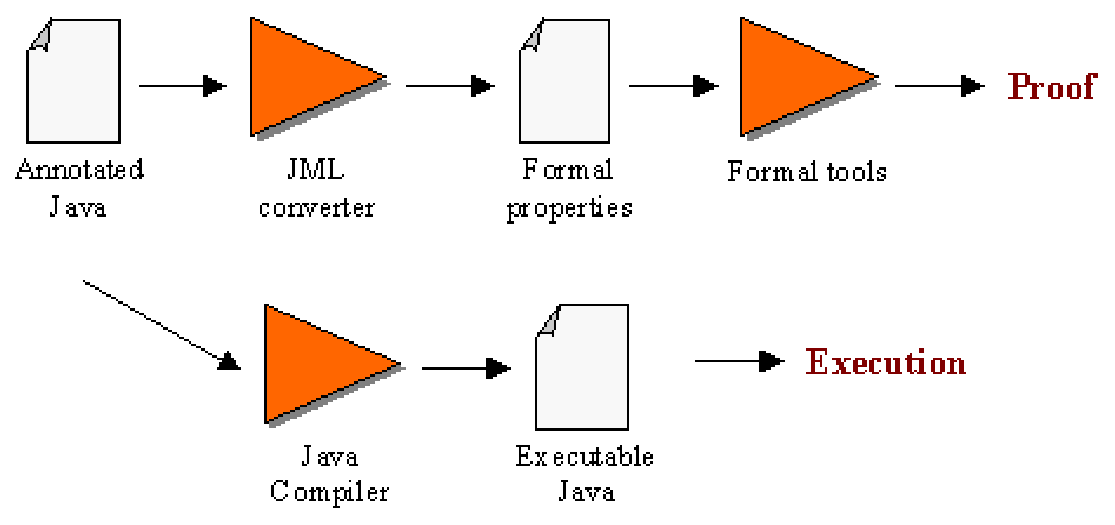
\psfig{file=fm03/image002.eps,width=14cm}
 \caption{\JACK\ architecture}
 \label{JACKarchitecture}
\end{figure}
 Figure \ref{JACKarchitecture} presents an overview of the \JACK\
 architecture.  \JACK\ consists of two parts: a converter (a lemma generator) from
 Java source annotated with JML into JPOL lemmas, and a viewer that
 allows developers to understand the generated
 lemmas.  The viewer is integrated in an IDE and is described more precisely in section
 \ref{Viewer}.  This part focuses on the converter.

 The \JACK\ converter converts a Java class into a JPOL model and allows to
 prove properties. 
 The initial goal was to prove properties on source files written with the Java
 language.  To reach this goal, one has to know how to ``translate'' a
 Java source file in formal lemmas.  

\begin{figure}[p]
 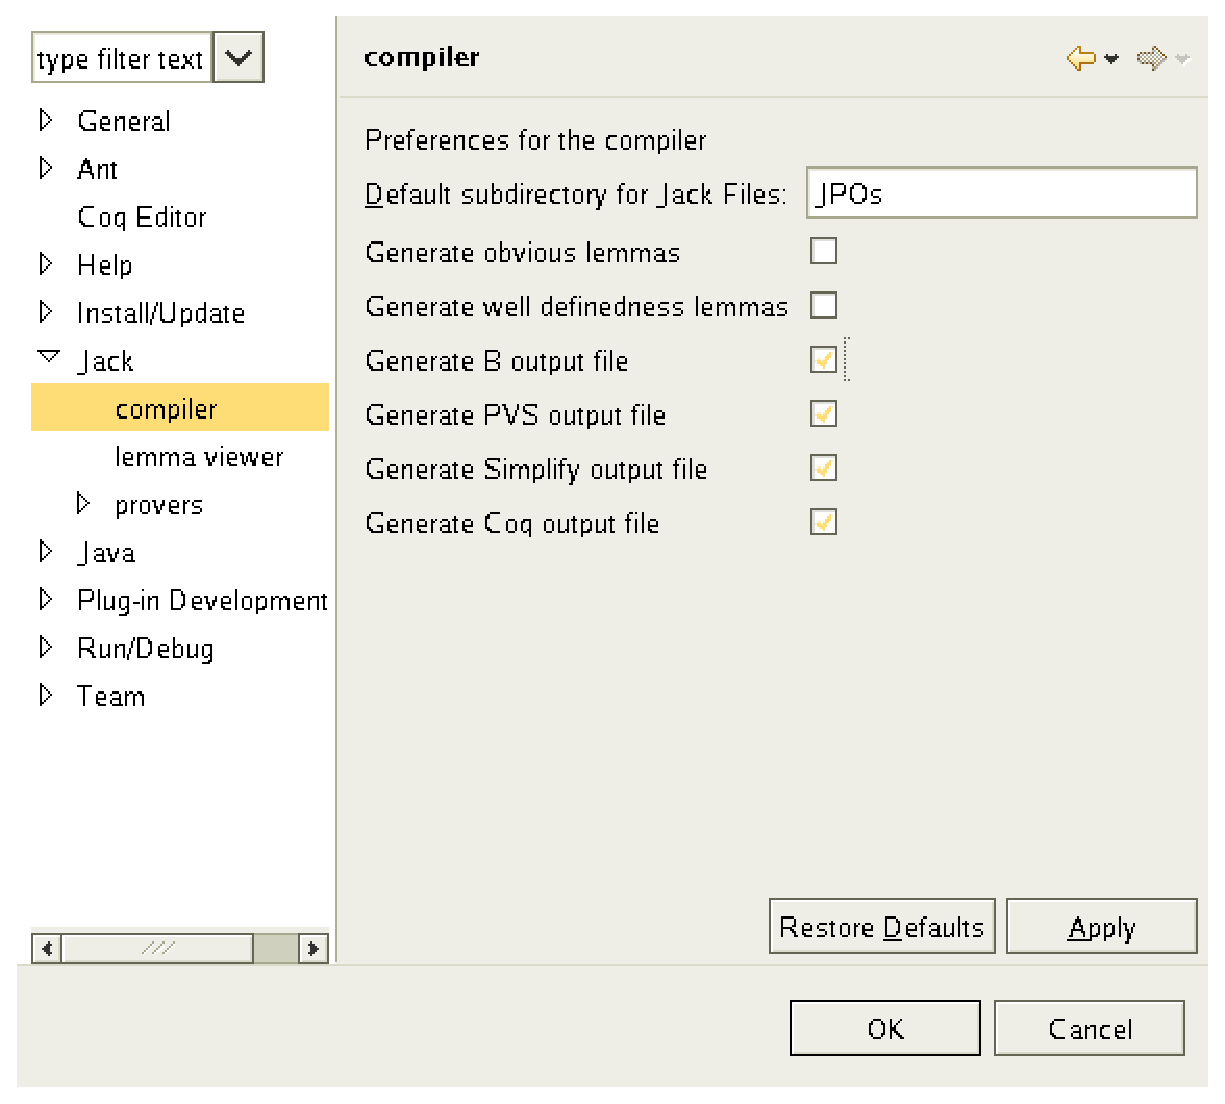
\psfig{file=fm03/preferences-compiler.eps,width=14cm}
 \caption{\JACK\ compiler preferences page}
 \label{JACKcompprefpage}
\end{figure}
 The JML annotations are Java boolean expressions without side
 effects.  Thus, they are easily translated in logical formulas: Java operators are
 translated into functions. For example, shift left (\texttt{<<}) is
 translated into a function associating an integer to a pair of
 integer.  From those translated annotations and the methods code,
 lemmas can be generated automatically.

 From the start, taking into account
 experiences in lemma generation for B machines, we have implemented a Weakest Precondition (WP) calculus to automate lemma
 generation.  Huisman, in \cite{Huisman:PhD}, presents how the
 classical Hoare logic can be completed to allow the generation of
 lemmas in the context of Java.  The Java statements contain different
 features like control-flow breaks.  So, the classical WP calculus
 should be completed to deal with them.

 Moreover, JML should be lightly upgraded to allow fully automated proof obligation generation.
 Notably, to
 automate lemma generation for the loops, we have had to extend
 the JML language with new keywords: \texttt{loop\_modifies}.
 The \texttt{loop\_modifies} keyword allows us to declare the variables modified in
the body of the loop, as it is done for the methods. During the WP calculus, it is necessary to universally
quantify the loop invariant with those variables, and since they cannot be automatically calculated, one has to
specify them.
 
 The two main drawbacks of the WP calculus are the loss of information and
 potential exponentional explosion.  After lemmas have been generated,
 it is often difficult to understand from which part of the code they
 are derived.  To bypass this issue, program flow information is
 associated to each lemma.  This information is used in the viewer
 to associate an execution path to each lemma. This feature is described in the next section.

 Exponentional explosion remains a problem.  Different solutions exist
 to avoid it.  As the WP calculus can be considered as a brute
 force concept, trying to expand all the path of the methods,
 solutions are always based on interaction to reduce this brute force
 by introducing intelligence in the process.

 A simple solution is to require users interaction during lemma
 generation in order to cut unsatisfiable branches.  Rather than introducing
 interaction during generation, another solution is to allow to add
 special annotations in the source code to introduce formulas that are
 taken into account at generation to simplify the lemmas.
 The solution adopted in \JACK\ is to allow to specify blocks. An exponentional explosion usually occurs
in a method with many sequenced branched statement ({\tt if, switch}, etc.) Such methods usually perform
different distinct sequenced treatments.
 Figure \ref{Specified_block} presents the skeleton of such a method. Specifying a block (here the second part
of the method) allows to cut proof obligation generation. This corresponds, in fact, to the simulation of a
method call.
\begin{figure}[htp]
{\tt
\begin{tabbing}
 \hspace{3 cm} \=m()\= \ \{ \\
 \> \> \vdots \\
 \> \> if () \{ $\hdots$ \} \\
 \> \> else \{ $\hdots$ \}   \\
 \> \> \vdots                   \\
 \> \> /*\=@ modifies {\it variables}  \\
 \> \> \> @ ensures {\it property} \\
 \> \> \> @\=*/ \{ \\
 \> \> \> \> \vdots \\
 \> \> \> \> if () \{ $\hdots$ \} \\
 \> \> \> \> else \{ $\hdots$ \}   \\
 \> \> \> \> \vdots                   \\
 \> \> \ \} \\
 \> \> \}
\end{tabbing}
}
 \caption{Specified block}
 \label{Specified_block}
\end{figure}

 With those extensions to the JML language, we are able to obtain a fully automated proof obligation generation.
That is the first step to reach user approval. The second one is to propose an access to those lemmas in a
``Java style'', this is described in the next section.

\subsection{User Interface}
\label{Industrialisation}
JML has the advantage of being a language that can be rapidly and
easily learned and used by developers. One can consider that using a
prover is not so easy. Nevertheless formal activities like modeling
and proving should not be reserved to experts. To demonstrate this
concept, we provide a prover interface understandable to non-experts
in formal methods.

In order to simplify the modeling activity with the JML language, our
interface requirements are:
\begin{itemize}
 \item to be integrated with other tools used by developers, and
 \item not to require the developer to use a mathematical formalism,
    but hide the mathematical formalism under a ``Java'' view.
\end{itemize}
Compared to other formal tools using the JML language, the efforts on
the user interface and integration within the development
environment is probably the main strength of \JACK, as is the fact
that the underlying mathematical formalism is not exposed to the
user.
\paragraph{Integration in developers environment}
 Java developers are used to develop using integrated development
 environments (IDE).  Those IDEs provide many features useful during
 the development process.  Integrating the tool in such IDEs allows
 the user to work in a familiar environment.  This leads both to
 better acceptance of the tool, and to a reduced learning curve.
 Currently, \JACK\ is integrated within the eclipse IDE.  It could
 however be ported to other IDEs, and a standalone version that does
 not require an IDE also exists.

 Another constraint has to be taken into account to obtain developer
 agreement: it is the tool's responsiveness.  The tool has to be used
 interactively, with a debugger spirit: it should not require the
 developer to wait for a long time.  Lemma generation takes, in
 realistic examples, less
 than one minute. %(see Section \ref{Case Study} for metrics).
 Nevertheless, the automatic proof of lemmas is not such a reactive
 activity. Thus, the tool provides a feature that allows to schedule
 proof tasks in order to optimize proof time (see paragraph
 \ref{Support for automatic proof}).


%Several other minor features are available to integrate within the
%development cycle, for example, reports on the status of the project
%can be generated as Microsoft Excel files.
\paragraph{Lemma Viewer}
\begin{figure}[p]
 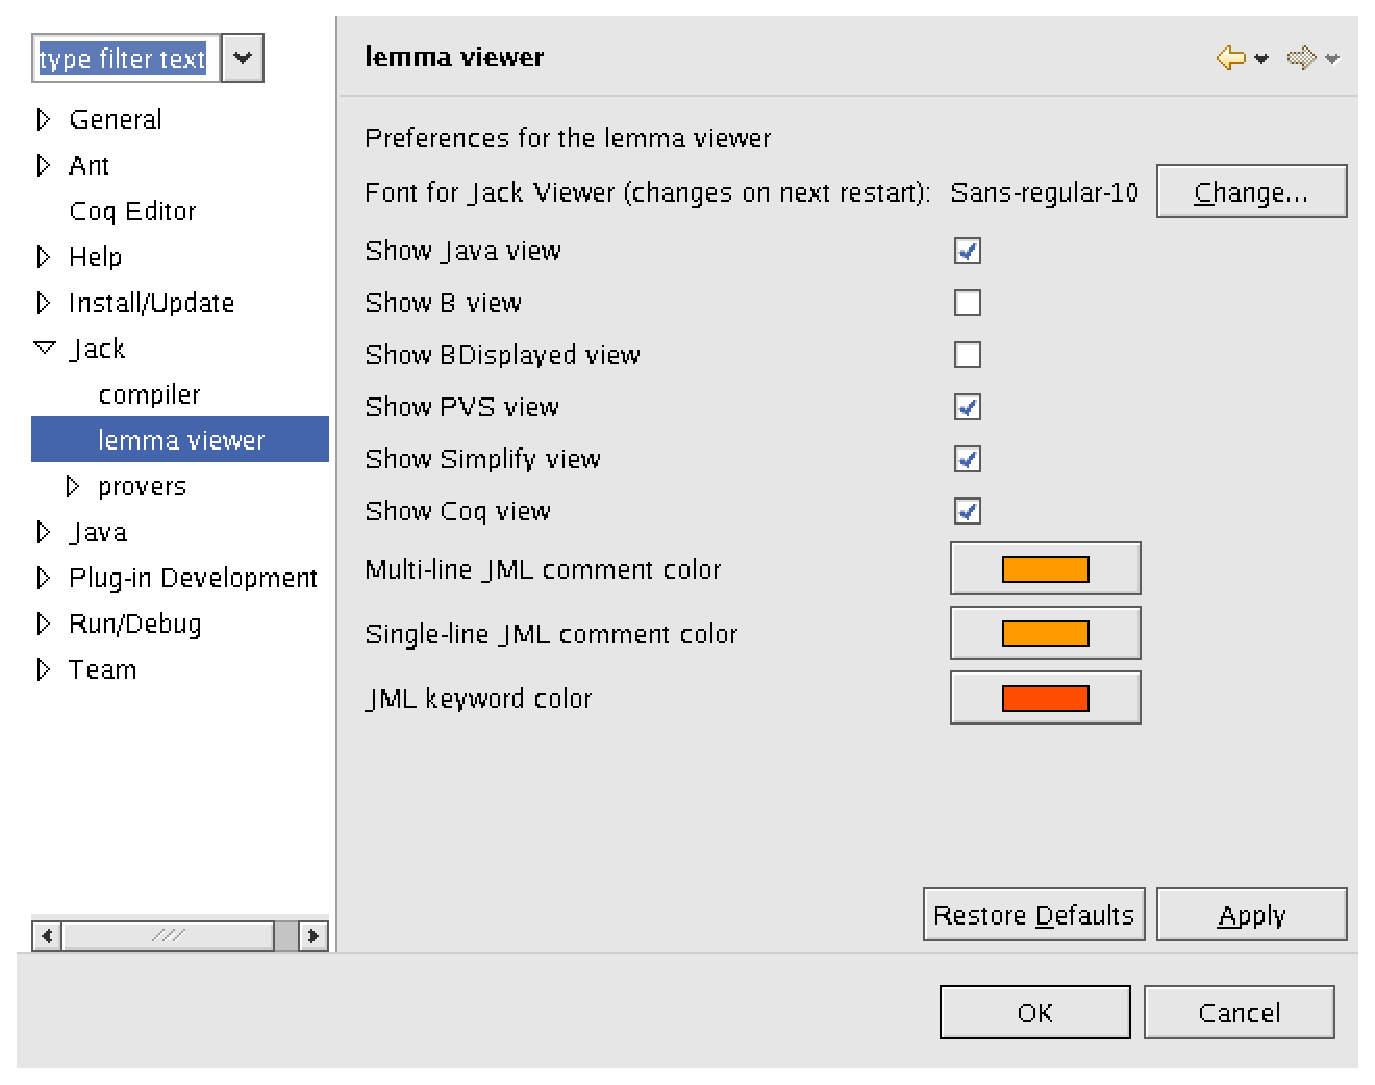
\psfig{file=fm03/preferences-editor.eps,width=14cm}
 \caption{\sc \JACK\ lemma viewer preferences page}
 \label{JACKlemviewprefpage}
\end{figure}
\label{Viewer}
One of the most important points of \JACK\ is that it does not require
developers to learn a mathematical language.  Although lemmas are
generated, those lemmas are not directly displayed to the user.

Instead, we provide the user with a graphical view (Figure \ref{Viewer image}) of the lemma.
 The viewer displays
 \begin{itemize}
  \item information concerning the current proof status;
  \item the class methods with their lemmas;
  \item the source code;
  \item and the currently selected lemma (goals and hypotheses with JPOL and prover language translations).
\end{itemize}
 Within a method, each execution path corresponds to a case.
 Possibly, several lemmas are associated to each case.
 When a case is selected, the corresponding execution path is highlighted.
 When a lemma is selected, its views are displayed.
\subparagraph{Path highlighting}
The source code of the program considered is displayed, and the
path within the program that leads to the generated proof obligation
is highlighted.

\begin{figure}[p]
 \epsfig{file=fm03/jack01.eps,width=15cm}
 \caption{\sc Viewer integrated in eclipse}
 \label{Viewer image}
\end{figure}

Different highlighting colors are used to represent this path:
\begin{itemize}
\item green indicates that the corresponding instruction has been
   executed normally;
\item blue indicates that the corresponding instruction has been
   executed normally, and that additional information is
   available. For instance, the condition of an \texttt{if} construct will
   usually be displayed in blue with additional information indicating
   if the condition has been considered as true or false;
\item red indicates that the corresponding instruction was supposed to
   raise an exception when it has been executed in the case
   considered.  Additional information are also provided indicating
   the exception that has been raised.
\end{itemize}
The part of the specification (invariant or post-condition) that is
involved in the current lemma is also highlighted.  Highlighting the
part of the source code involved in the proof obligation allows to
quickly understand the proof obligation, and allows the user to treat
the proof obligations as execution scenarios of the program.
\subparagraph{Java presentation of lemmas}
The hypothesis and goals of the current lemma are also displayed. As
the conversion mechanism into provers language may be hard to follow, especially by
non-experts, the internal representation used by the tool is used to
present the hypothesis and goals in a Java representation. That is,
all the variables are displayed using the Java dotted notation, and
the Java operators are used instead of their corresponding function.

However, such a translation may be more complicated when operators that
have no Java or JML equivalent constructs are used.  


 However, although the Java view is able to handle some internal
 representation constructs that do not have direct Java or JML
 equivalent constructs, there are still constructs that cannot be
 translated, and for which a Java notation is hard to define. For
 instance some set operators cannot be translated in a generic way.

\subsubsection{Support for verification}
Apart from displaying the generated proof obligations, \JACK\ also
provides support for validating those proofs, as detailed hereafter.
\subparagraph{Support for automatic proof}
\label{Support for automatic proof}
 A point that should not be taken lightly is the time taken by
automatic proof: generating proof obligations for industrial size
applications will generate thousands of proof obligations.

Typically, those proofs can be quite lengthy, and it is necessary that
the user is not obliged to wait for proofs to finish.

To achieve this, \JACK\ provides an independent proof view, where
files can be queued in order to be submitted to the prover. Thus, the
proofs are performed as soon as possible, possibly during the night,
allowing the user to focus on cases inspection.

\subparagraph{Support for interactive proof}
Although the automatic prover allows discharging many proof
obligations, it cannot discharge all the proof obligations. Thus, the
remaining proof obligations have to be verified manually.

Currently, developers are not supposed to handle this task, but to
delegate it to a team of experts that would perform the proofs using
the interactive prover of the \texttt{Atelier B} tool, emacs with PVS
or the Coq editor.


\subparagraph{Checking proof obligations}
Additionally to the ``\textit{proved}'' and ``\textit{unproved}''
states, \JACK\ can also differentiate ``\textit{checked}'' proof
obligations. Checked proof obligations correspond to proof obligations
that are not formally proved, but have been manually verified.

Checking proof obligations is performed by the user to indicate that
he has read and understood the proof obligation and has confidence
that it is correct. Although the checked state provides no formal
guarantee on the correctness of the proof obligations, it still
provides valuable information on the state of a project.

The checked state of the proof obligations can be used in different
ways:
\begin{itemize}
\item To flag cases as already seen in order to start an interactive
   proof only if we are pretty sure that the cases are correct, and
\item In some cases, when a full correctness assurance of the program is not
   required, we may accept that not all the proof obligations are
   formally proved. In that case, it may however, be required that all
   the proof obligations have been checked.
\end{itemize}
In order to minimize verification time, one can assure that checked
proof obligations remain unchanged through subsequents runs of the
proof obligation generator---otherwise the time spent to inspect the
proof obligation and to ensure manually that it is correct would be
lost. 


\subsection{Case study}
\label{Case Study}
% Tableau avec chiffres, etc...
To test \JACK, we have developed a little banking application.  This section presents different metrics
concerning the evaluation of the tool on this package.
\begin{table}
 \begin{tabular}{|l|c|c|c|c|c|c|c|} \hline
 Classes & Java & JavaDoc & JML & Proof & Automatic & Time to PO & Time to \\
  & lines & lines & lines & obligations & proof & generate (s) & prove (s)\\  \hline
 Transfert\_src  & 116 & 34 & 150 & 359 & 91\% & 22,5 & 238 \\
 AccountMan\_src & 105 & 51 & 236 & 269 & 82\% & 12,7 & 195 \\
 Currency\_src   &  93 & 20 &  28 &  50 & 96\% &  7,6 &  17 \\
 Balance\_src    &  64 & 38 &  58 & 335 & 95\% & 16,5 & 191 \\
 Spending\_rule  &  40 & 33 &  62 &  42 & 67\% & 13,6 & 217 \\ \hline
 \end{tabular}
\caption{banking applet metrics}
\label{MetricsTable}
\end{table}
Different remarks can be made from Table \ref{MetricsTable}, concerning the cost of adding JML annotations, the
performance of the tool, as well as the cost associated to the proof.
\paragraph{Cost of the annotations}
A first remark concerns the cost of the annotations.  The metrics given here only concern the number of lines
but one can see that the documentation size (JavaDoc and JML) is one and half greater than the code size.  So,
writing  the JML specification seems to be a costly activity.  This remark can be moderated by two points: this
development was the first that we made, and annotations were added to already existing code. So it suffers from
its lack of abstraction, and the annotations are really verbose. Moreover the time to specify is to be compared
to the time to develop test data.
\paragraph{Responsiveness}
The automatic phases are quite responsive with some seconds to generate proof obligations.  The automatic proof
is not as cheap as the proof obligation generation and takes a few minutes. However, this still remains
acceptable, since it is a non-blocking task that does not require users to wait for its completion.

For larger applets, it is however expected that the time required for the automatic proof will significantly
increase.
\paragraph{Proof}
The automatic proof rating is much good.  It is quite greater than the usual value for a B development (around
80\%).  This is mainly due to the fact that we used this applet as a test applet for extending the prover. So,
as a side effect, the automatic prover is customized for this special applet.

Nevertheless, after automatic proof step, there remain 111 lemmas to prove using the Atelier B interface.  An
expert needs between 4 and 5 days to prove them.

\subsection{Perspectives}
\label{Perspectives}
 At the moment, we have developed a prototype that is becoming a
 usable tool.  We are beginning experimentation outside the lab.  But
 we are considering that there are still many points where the
 approach can be improved.
%\subsection{JML Subset considered}
% JACK currently handles a subset of JML corresponding to lightweight
% specifications.  Future work should improve that subset by allowing
% to use a larger subset of JML including full fledged behavior
% specifications and pure method calls.

\subsubsection{Interactive proof cost}
 Currently, the interactive proof support is rather limited.  Thus,
 proving the remaining proof obligations requires users to directly
 use the \texttt{Atelier B} tool interactive prover.  Such a task can
 be tedious, since the B representation of the generated proof
 obligations can be hard to follow.  Different perspectives exist to
 reduce the interactive proof cost.

% AR: remplac� non-expert par Java: en effet je trouve que �a serais
% plus pratique m�me pour un expert.
\paragraph{Java interface}
 Although full interactive proof will still be reserved to experts,
 providing an interface to the \texttt{Atelier B} interactive prover
 allowing to perform proofs by directly using the Java syntax would
 greatly improve the productivity of those experts.  A first step
 would be to extend the Java view used to display the lemmas.

\paragraph{Test Activity}
 Another way to reduce interactive proof activity is to balance it
 with testing activity.  Methods where lemmas are not automatically
 proved could be tested.  Using \texttt{JmlJunit} can be a good way to
 generate test skeleton on certain cases.  A perspective is to
 integrate \texttt{JmlJunit} in our environment in manner to propose
 different validation level (full proof, proof mixed with test, etc).

\paragraph{Counter-example}
 Another idea to reduce the cost of false lemma detection is to
 provide counter-example when it is possible.  \ESC\ already tempts to
 give such counter-examples.  Studies on that subject could give
 results helpful for developers to understand errors on the code or on
 the specifications.

\subsubsection{Allowing expressions in the target formal language}
Currently, \JACK\ can be seen as a proof-obligations generator from
JML annotated Java programs to B lemmas.  A possible extension would
be to add different target languages for lemma generation, for
instance Coq or PVS. Such extension would allow using different
provers for different lemmas.  On the other side, it is also possible
to enrich the JML specification by adding inline expressions or
variables in a target language of the lemma generator. 
Such an extension would have a role similar to Java ``native methods''
at a specification level. That is, allowing to describe in a
lower-level language things that cannot be described in JML (or that
cannot be described efficiently from a proof point of view).

We are currently investigating such extension mechanisms, that would
allow adding different languages for such use without having to modify
the weakest-precondition calculus core.

\subsection{Conclusion}
\label{Conclusion}
 The presented work allows formal methods experts to prove Java applet correctness.
 Moreover, it allow Java programmers to obtain an high assurance on their code correctness.
 This leads to the most important point:
it allows non-experts to venture into the formal world.  This is a necessary starting point for such validation
techniques to be widely used.

  The tool has been developed following a main
 objective: let Java developers validate their own code.  We claim
 that JML is well suited to express low level design and conception
 choices and that usage of \JACK\ can replace effectively unitary tests,
 giving developers the means to furnish code with good quality
 and non ambiguous documentation.

 Taking benefits from recent research on Java program validation, we have
 developed an automated tool that generates lemmas from Java classes
 annotated with JML.
 The \JACK\ principles are not really different from the \LOOP\
 team choices.  Nevertheless, one can highlight some important
 differences.
 The \LOOP\ tool describes formally Java semantics and the WP-calculus rules are applied by the prover.
 The main advantage is that the rules have been proven sound with regards to the semantics in the theorem prover.
 Our point of view, is more pragmatic: lemma are generated automatically, using
 Java developed rules that can only be checked by usual validation: test, code-inspection.
 The soundness of the tool cannot be formally proved but on the other hand a big effort is done to present
 lemmas to users in a way that he can understand them and verify
 that they are valid.

 The tool is fully integrated in the eclipse IDE
 and presents lemmas in a visual way that allows developers to form their
 opinion on the lemma validity.  An automatic prover discharges an
 important part of the lemmas.  The remaining lemmas have to be proved
 using the prover interface.  Often, this task cannot be done by developers.
 Different ways are studied to bypass it: expert support, test case
 generation, counter-example detection, etc.

 We are now experimenting on real industrial products.  We are
 trying to collect metrics in order to prove that this kind of
 validation is cost-saving, especially when the cost of testing is
 taken into account.


\section{Security property propagation}

%\input BML/cmdBML.tex

\newcommand{\code}{\textit{code}}
\newcommand{\indexComp}{\textit{index}}





\section{Introduction} \label{bcsl}
This section presents a bytecode level specification language, called for short BML and a compiler from a
 subset of the high level Java specification language JML to BML. 

% motivation

 Before going further, we discuss what advocates the need of a low level specification language.
Traditionally, specification languages were tailored for high level languages.  
Source  specification allows to express complex functional or security properties about programs.
Thus, they are / can successfully be used 
for software audit and validation. Still, source specification in the context of mobile code does not help a lot for several reasons.


First, the executable / interpreted code  may not be accompanied by its specified  source. Second, it is more reasonable for the 
code receiver to check the executable code than its source code, especially if he is not willing to trust the compiler. 
Third, if the client has complex requirements and even if the code respects them, in order to establish them, 
the code should be specified. Of course, for properties like well typedness this specification can be inferred automatically,
but in the general case this problem is not decidable. 
Thus, for more sophisticated policies, an automatic inference will not work.

 It is in this perspective, that we propose to make the Java
bytecode benefit from the source specification by defining the BML language and a compiler from JML towards BML.    

% what does the language support?
 BML supports the most important features of JML. Thus, we can express functional properties of Java
 bytecode programs in the form of method pre and postconditions, class and object invariants, assertions
 for particular program points like loop invariants. To our knowledge BML does not have predecessors that are tailored 
 to Java bytecode.  

 In section \ref{BCSLprelim}, we give an overview of the main features of JML. A detailed overview of BML is given in section \ref{BCSLgrammar}.  
  As we stated before, we support also a compiler from the high level specification language JML into BML. The 
 compilation process from JML to BML is discussed in section  \ref{BCSLcompile}.
 The full specification of the new user defined Java attributes in which the JML specification is compiled is given in the appendix.





\subsection{High-level Security Properties for Applets}
\label{SecHighLevelSecProp}

The properties that we consider can be divided in several groups,
related to different aspects of smart cards. First of all there are
properties dealing with the so-called \emph{applet life cycle},
describing the different phases that an applet can be in. Many actions
can only be performed when an applet is in a certain phase. Second,
there are properties dealing with the transaction mechanism, the Java
Card solution for having atomic updates. Further there are properties
restricting the kind of exceptions that can occur, and finally, we
consider properties dealing with access control, limiting the possible
interactions between different applications. For each group we present
some example properties. For all these properties encodings into JML
annotations exist.

\paragraph {Applet life cycle}

A typical applet life cycle defines phases as {\it loading},
{\it installation}, {\it personalization}, {\it selectable},
{\it blocked} and {\it dead}
(see \emph{e.g.}~\/\cite{MarletLM01}).  Each phase corresponds to a
different moment in the applet's life. First an applet is loaded on
the card, then it is properly installed and registered with the Java
Card Runtime Environment. Next the card is personalized,
\emph{i.e.}~all information about the card owner, permissions, keys
\emph{etc.} is stored. After this, the applet is selectable, which means
that it can be repeatedly selected, executed, and deselected. However,
if a serious error occurs, for example there
have been too many attempts to verify a pin code, the card can get
blocked or even become dead. From the latter state, no recovery is
possible.

In many of these phases, restrictions apply on who can perform
actions, or on which actions can be performed. These restrictions give
rise to different security properties, to be obeyed by the applet.

\begin{quote}
\textbf{Authenticated initialization} Loading, installing and 
personalizing the applet can only be done by an authenticated
authority.\smallskip\\
\textbf{Authenticated unblocking} When the card is blocked,
only an authenticated authority can execute commands and possibly
unblock it.\smallskip\\
\textbf{Single personalization} An applet can be
personalized only once.
\end{quote}


\paragraph {Atomicity}

A smart card does not include a power supply, thus a brutal retrieval
from the terminal could interrupt a computation and bring the system in
an incoherent state. To avoid this, the Java Card
specification prescribes the use of a transaction mechanism to
control synchronized updates of sensitive data. A 
statement block surrounded by the methods \texttt{beginTransaction()} and
\texttt{commitTransaction()} can be considered atomic.
If something happens while executing the transaction (or if
\texttt{abortTransaction()} is executed), the card will
roll back its internal state to the state before the transaction was
begun.

To ensure the proper functioning and prevent abuse of this mechanism,
several security properties can be specified.

\begin{quote}
\textbf{No nested transactions} Only one level of transactions
is allowed.\smallskip\\
\textbf{No exception in transaction} All exceptions that may be thrown
inside a transaction, should also be caught inside the
transaction.\smallskip\\
\textbf{Bounded retries}
No pin verification may happen within a transaction.
\end{quote} 
The second property ensures that the \texttt{commitTransaction} will
always be executed. If the exception is not caught, the
\texttt{commitTransaction} would be ignored and the transaction would
not be finished. The last property excludes pin verification within a
transaction. If this would be allowed, one could abort the transaction
every time a wrong pin code has been entered. As this rolls
back the internal state to the state before the transaction was
started, this would also reset the retry counter, thus allowing an
unbounded number of retries. Even though the specification of the Java
Card API prescribes that the retry counter for pin verification cannot
be rolled back, in general one has to check this kind of properties.

\paragraph{Exceptions}

Raising an exception at the top level can reveal
information about the behavior of the application and in principle it
should be forbidden. However, sometimes it is necessary to pass on
information about a problem that occurred. Therefore, the Java
Card standard defines so-called ISO exceptions, where a pre-defined
status word explains the problem encountered. These exceptions are the
only exceptions that may be visible at top-level; all other exceptions
should be caught within the application.

\begin{quote}
\textbf{Only ISO exceptions at top-level}
No exception should be visible at top-level, except ISO
exceptions.
\end{quote}

\paragraph {Access control} 

Another feature of Java Card is an isolation mechanism between
applications: the firewall. The firewall ensures that several
applications can securely co-exist on the same card, while managing
limited collaboration between them: classes and interfaces defined in
the same package can freely access each other, while external classes
can only be accessed via explicitly shared
interfaces. Inter-application communication via shareable interfaces
should only take place when the applet is selectable, in all other
phases of the applet life cycle only authenticated authorities are
allowed to access the applet. 
\begin{quote}
\textbf{Only selectable applications shareable} An application is accessible
via a shareable interface only if it is selectable.
\end{quote}


\subsection{Architecture}

\begin{figure}[pht]
\begin{center}
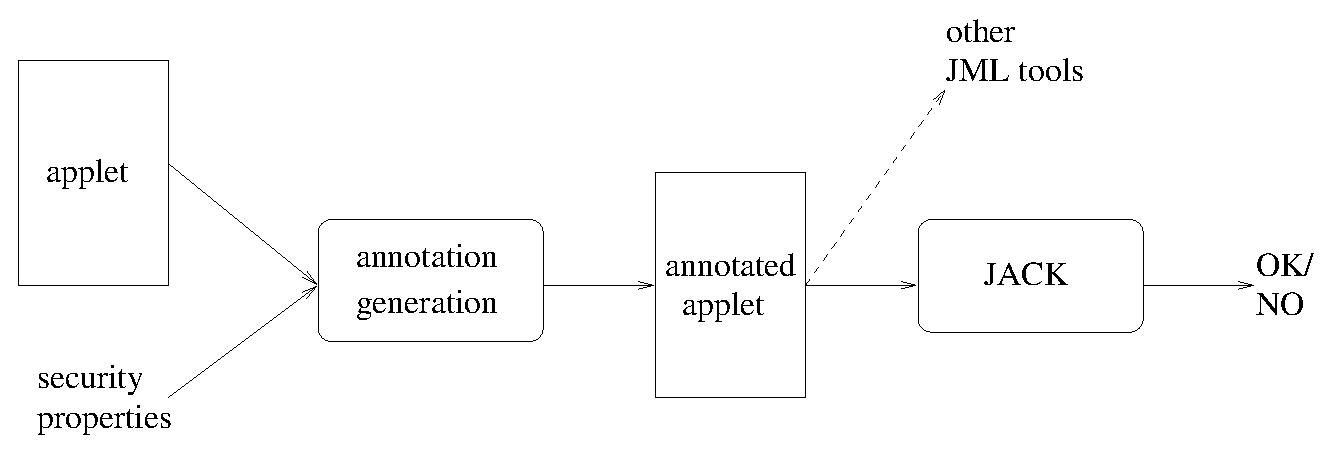
\epsfig{file=isaac/architecture.eps, width=9cm}
\end{center}
\caption{\sc Tool set for verifying high-level security properties}\label{FigArch}
\end{figure}



Figure~\ref{FigArch} shows the general architecture of the tool set
for verifying high-level security properties. Our annotation generator
can be used as a front-end for any tool accepting JML-annotated Java
(Card) applications. As input we have a security property and a Java
Card applet. The output is a JML Abstract Syntax Tree (AST), using the
format as defined for the standard JML parser. When pretty-printed,
this AST corresponds to a JML-annotated Java file. From this
annotated file, JACK generates appropriate proof obligations to check
whether the applet respects the security property.

\subsection{Automatic Generation of Annotations}

The propogation consists mainly on a weaving phase,
\emph{i.e.}~how the core-annotations are propagated throughout the
applet. We define functions \textsf{mod}, \textsf{pre}, \textsf{post} and
\textsf{exc\-post}, propagating assignable clauses, preconditions, 
postconditions and exceptional postconditions, respectively. These
functions have been defined and implemented for the full Java Card
language, but to present our ideas, we only give the definitions for a
representative subset of statements: statement composition, method
calls, conditional and \texttt{try}-\texttt{catch} statements and
special set-annotations. We assume the existence of domains
\textsf{MethName} of method names, \textsf{Stmt} of Java Card
statements, \textsf{Expr} of Java Card expressions, and \textsf{Var}
of static ghost variables, and functions
\textsf{call} and \textsf{body}, denoting a method call and 
body, respectively.

All functions are defined as mutual recursive functions on method
names, statements and expressions. When a method call is encountered,
the implementation will check whether annotations already have been
generated for this method (either by synthesizing or weaving). If not
it will recursively generate appropriate annotations. Java Card
applets typically do not contain (mutually) recursive method calls,
therefore this does not cause any problems. Generating appropriate
annotations for recursive methods would require more care (and in
general it might not be possible to do without any user interaction).



\section{Comparison between source and bytecodes \\ proofs}  \label{results}

The purpose of this section is to give a comparison between bytecode and source proof obligations.
In particular, we illustrate this by the proof obligations of the example program in Fig.\ref{replaceSrc}.
%We have an implementation of the JML compiler ( subsection \ref{comJML}) and the bytecode verification condition generator based on the weakest precondition calculus (Section \ref{wpbc}) which are integrated in JACK. Both of the verification condition generators perform the same simplifications over the verification conditions 
%, e.g. eliminate verification conditions that contain contradictory hypothesis or trivial goals (equal to true). 

%The performed tests show that JML compilation augments around twice the file size. 
%For the example in Fig.~\ref{replaceSrc}, the class file without the specification extensions is 548 bytes, 
%and the class with the BCSL extension BCSL is 954 bytes. 
%The size of the bytecode specification is proportional to the source specification: 
%the bigger is the source specification, the greater will be the size of the class file. 
We studied the relationship between the source code proof obligations generated 
by the standard feature of JACK and the bytecode proof obligations generated by our implementation over the corresponding bytecode
 produced by a non optimizing compiler over the examples given in \cite{JPVC03JKM}. The proof obligations were the same modulo 
program variables names and basic types.

 We return now to our example from the previous sections and give in Fig. \ref{vcEnsures} one of the proof obligations on source 
and bytecode level respectively concerning the postcondition correctness. The verification conditions on bytecode and source level
 have the same shape modulo names (see Section \ref{comJML} for how names are compiled). Also in Section
 \ref{comJML}, we discussed the compilation of the JML postcondition from Fig. \ref{replaceSrc}. Particularly,
 we saw that the compiler has to transform the source postcondition in an equivalent formula and we
 gave the compilation in Fig. \ref{postCompile}. 

Despite those transformations, the source and bytecode goal respectively (which are actually the postcondition) on bytecode and source level are not only
semantically equivalent but syntactically the same (except for the variable names ). Still, in the bytecode proof obligation we have one more hypothesis than on source level. The extra hypothesis in the bytecode proof obligation is related to the fact that the result type is boolean but the JVM encodes boolean expressions as integers (which is trivially true). This means that the proof obligations have also the same shape.

 Another important issue is the impact of simple optimizations like dead code elimination on the relationship between source and bytecode proof obligations. 
In this case, the compiler does not generate the dead code and the bytecode verification condition generator will neither ``see'' it. 
Even though the source contains the never taken branch as the condition is equivalent to false, this will result in a trivially true
verification condition which the JACK source verification condition generator will discard.

The equivalence between source and bytecode proof obligations can be exploited in PCC scenarios, as we discussed in Section \ref{architecture} where 
the producer generates the program certificate over the source code in scenarios where a complete automatic certification (e.g. the certifying compiler) will not work.
 
We aim to formally give evidence that the proof obligations on non optimized bytecode and source programs are syntactically the same (modulo names and types). 

%Fig. \ref{vcLoopPreserv} shows the proof obligations for the loop preservation. As you can see the hypothesis and the goal have the same ``shape'' on bytecode and source code and the differences are due to the variable names.



% \begin{figure}{!h}

% $$\begin{array}{ll}
%Hypothesis \ on \ bytecode:  & Hypothesis \ on \ source \ level:  \\
%% & \\

%
%\begin{array}{l}
% \register{1} \neq \\
%\#19 (\register{0})[\register{2}\_at\_ins\_22]
%\end{array}  
%
%&  
%\begin{array}{l}
% \srcVar{obj} \neq \\
%  ListArray.list(\this)[\srcVar{i}\_at\_ins\_26] 
%\end{array}   \\
%
%
%
% & \\
%
%\#19(\register{0}) \neq \Mynull &  ListArray.list( \this) \neq \Mynull\\
%
%
%& \\
%
%\begin{array}{l}
%  len(\#19 (\register{0})) > \\
% \register{2}\_at\_ins\_22 
%\end{array}
%%& 
%\begin{array}{l}
%  len(ListArray.list(\this)) > \\
%\srcVar{i}\_at\_ins\_26
%\end{array}         \\ 

%

% & \\
%
% \register{2}\_at\_ins\_22 \geq 0 &   \srcVar{i}\_at\_ins\_26    \geq 0    \\
%
%
% & \\
%\begin{array}{l}
%  \register{2}\_at\_ins\_22 < \\
%  len(\#19(\register{0}))
%\end{array} &
%
%\begin{array}{l}
%  \srcVar{i}\_at\_ins\_26 <\\
%  len(ListArray.list(\this))
%\end{array}   \\
%
%
% & \\
%\begin{array}{l}
%  \register{2}\_at\_ins\_22 \leq \\
%  len( \#19(\register{0}))
%\end{array} 
%&  
%\begin{array}{l} 
%  \srcVar{i}\_at\_ins\_26 \leq \\
%  len(ListArray.list(\this))
%\end{array}   \\
%
%
% &\\
%% \register{2}\_at\_ins\_22 \geq 0 &   \srcVar{i}\_at\_ins\_26 \geq 0 \\
%
%
%
%% &\\
% \begin{array}{l} 
%         \forall  var(0). \ 0 \leq var(0) \wedge var(0) < (\register{2}\_at\_ins\_22) \Rightarrow \\
%                \Myspace    \#19(\register{0})[var(0)] \neq \register{1}
%      \end{array} &        
%      \begin{array}{l} 
%             \forall  var(0). \ 0 \leq var(0) \wedge var(0) < (\srcVar{i}\_at\_ins\_26) \Rightarrow \\
%                 \Myspace       ListArray.list(\this)[var(0)] \neq \srcVar{obj}
%      \end{array}  \\
%%
% typeof(\register{0}) <: ListArray &    typeof(this) <: ListArray     \\
%
%& \\
%& \\
%Goal \ on \ bytecode: & Goal \ on \ source \ level: \\
%
%& \\
%
%  \begin{array}{l}
%               1 + \register{2}\_at\_ins\_22 \leq  len(ListArray.list(\register{0}))  \\
%
%               1 + \register{2}\_at\_ins\_22 \geq 0 \\
%
%               \forall  var(0). 0 \leq var(0) \wedge var(0) < 1 + \register{2}\_at\_ins\_22 \Rightarrow \\
%                   \Myspace  ListArray.list(\register{0})[var(0)] \neq \register{1} 
%
%       \end{array}
%& 
%
%       \begin{array}{l}
%             1 + \srcVar{i}\_at\_ins\_26 \leq  len(ListArray.list(this))  \\
%	     \\
%             1 + \srcVar{i}\_at\_ins\_26 \geq 0 \\
%	     \\
%             \forall  var(0). 0 \leq var(0) \wedge\\
%	     \Myspace  var(0) < 1 + \srcVar{i}\_at\_ins\_26 \Rightarrow \\
%                  \Myspace  ListArray.list(this)[var(0)] \neq \srcVar{obj} 
%       \end{array}   
%
 
%\end{array}$$



%\caption{Source and Bytecode verification condition for loop preservation for method \texttt{ListArray.isElem} }
%\label{vcLoopPreserv}
%\end{figure}








\begin{figure*}[!h]

\begin{center}
\begin{tabular}{|l|l|}
\hline
\bf{Hypothesis \ on \ bytecode:}  & \bf{Hypothesis \ on \ source \ level:}  \\
\hline 
$\register{2}\_at\_ins\_20 \geq $ 
& $ \srcVar{i}\_at\_ins\_26 \geq$ \\

$len(\#19(\register{0})) $ & $  len(ListArray.list(\this)) $ \\
\hline 

$\#19(\register{0}) \neq \Mynull$ 
& $ ListArray.list(\this) \neq \Mynull$ \\

\hline 
$ \register{2}\_at\_ins\_20) \leq$ 
&  $  \srcVar{i}\_at\_ins\_26  \leq   $ \\
$ len(\#19(\register{0}))  $ & $ len(ListArray.list(\this))  $ \\
\hline

$\register{2}\_at\_ins\_20 \geq 0  $ 
& $ \srcVar{i}\_at\_ins\_26  \geq 0 $ \\

\hline

$\forall  var(0). \  0 \leq var(0) \wedge  $ & $\forall  var(0). \  0 \leq var(0) \wedge $ \\
$ var(0) < \register{2}\_at\_ins\_20 \Rightarrow $ & $  var(0) < \srcVar{i}\_at\_ins\_26 \Rightarrow $\\
$ \#19(\register{0})[var(0)] = \register{1}   $ & $  ListArray.list(\this)[var(0)] = \srcVar{obj}  $ \\

\hline

 $typeof(\register{0}) <: ListArray$ & $typeof( \this) <:  ListArray$  \\
\hline

$0=0 \vee 0=1$ & \\

& \\

\hline
\bf{Goal on bytecode:} & \bf{Goal on source level:} \\
\hline
$\Myfalse  \iff $ & $\Myfalse \iff  $ \\
 $ \exists  var(0) . \ 0 \leq var(0) \wedge$ 
& $ \exists  var(0) . \ 0 \leq var(0) \wedge$ \\

$\Myspace \Myspace var(0) < len(\#19(\register{0})) \wedge$ 
& $\Myspace \Myspace  var(0) < len(ListArray.List(this)) \wedge $\\
       
$\Myspace \Myspace \#19(\register{0})[var(0)] = \register{1} $ 
&$\Myspace \Myspace  ListArray.List(this)[var(0)] = \srcVar{obj}  $ \\

\hline
\end{tabular}
\end{center}

Note: $\expression\_at\_ins\_n$ denotes the value of  
expression $\expression$ at the bytecode instruction at index (source line)  $n$ 

\caption{\sc Comparison of source and bytecode verification conditions}
\label{vcEnsures}
\end{figure*}

\clearpage
 















%\subsubsection{Example}
% We give a simple example of how the \wpi \ works. Block $\blockm{6}$ (starts at instr. \texttt{6}) in Fig.~\ref{blockBC} ends with a branching instruction and in the case when the condition is true (the current element of the array is not equal to the first parameter of the method \texttt{replace}) the execution will continue at $\blockm{19}$. Below we give the part of the weakest precondition for block $\blockm{6}$ in case the control flows to block $\blockm{19}$( the condition of its last instruction holds and in this case 
%the predicate $pre(b^{6}, b^{19})$ is $\wpi(\blockm{19})$).  The implications with conclusion \Myfalse \ stand for the possible exceptions \texttt{NullPointer} and \texttt{ArrayIndexOutOfBound} exceptions that may be thrown (as no postcondition is specified explicitly for these cases of abnormal termination, the one by default is taken). 

%\input wpExample.tex

%In this paper we focus on a verification framework adapted for the
verification of AspectJ programs annotated with Pipa.  The pointcut
semantic of AspectJ has been properly
defined~\cite{DBLP:conf/popl/AvgustinovHOMSTV07} as well as the advice
weaving semantic~\cite{weaving04} though only parts have been
formalized~\cite{weaving06}.  Pipa is an annotation language which was
inspired by Clifton and Leavens' work~\cite{clifton02observers}. There
are some extensions to it like pointcuts
annotations~\cite{pointcuts07}, or Moxa \cite{moxa05}.  Our framework
relies on verification based on an intermediate language, like what is
done in ESC/Java2~\cite{FlanaganLLNSS02}, Boogie~\cite{BarnettCDJL05},
or Krakatoa~\cite{MarcheP-MU04}. The work is made to be adapted on a
BoogiePL-like guarded command which is coupled with a
VCGen~\cite{BarnettL05,FlanaganS01}.

\paragraph{Modular verification of Aspects}
Verification in Aspect Oriented Programming language is often linked
to a modular approach.  It is orthogonal to the aim of this paperh: we
tailor verification of aspects which were not specially wanted by the
user, and are most-likely imposed by the environment.  Clifton and
Leavens~\cite{clifton02observers,clifton02spectators,cliftonPhd}
propose a programming discipline to define and specify aspects, using
an extension of JML as specification language.  They define two kind
of aspects, the \emph{spectators} and \emph{assistants} and propose to
explicitly allows the weaving of these aspects. This approach allows
efficient modular reasonning and easy implementations because they
show a way of weaving specifications using a control-flow graph
analysis. In their 2004 work~\cite{shriram04} Krishnamurthi {\it et
al} present a model-checking framework for verification of programs
containing aspects. It is quite different from our work as it presents
a generic framework for aspects. In an unpublished paper~\cite{cesar},
Kunz presents a Hoare logic for modular verification of aspects. The
paper is quite formal, but he does not add special annotations for method
specifications as Clifton and Leavens. For this reason his approach remains 
less modular than Clifton's, but more expressive.




% Shmuel Katz et al. \cite{Katz06,GoldmanK06} propose
% a classification of aspects as \emph{spectative}, \emph{regulative} or
% \emph{invasive}, to simplify program verification by focusing on the








\section{Conclusion and Future Work}\label{conclusion}
This article describes a bytecode weakest precondition calculus applied to a bytecode specification language (BCSL).
BCSL is defined as suitable extensions of the Java class file format.
Implementations for a proof obligation generator and a JML compiler to BCSL have been developed and are part of the Jack 1.8 release\footnote{http://www-sop.inria.fr/everest/soft/Jack/jack.html}.
At this step, we have built a framework for Java program verification.
 This validation can be done at source or at bytecode level in a common environment: for instance, to prove lemmas ensuring bytecode correctness all the current and future provers plugged in Jack can be used.

We are now aiming to complete our architecture for establishing trust in untrusted code - in particular extending the present work to a PCC architecture for establishing non trivial requirements.  
%Properties that can be verified are properties expressible in the JML specification language. Design by contract properties (used in interface design) can be easily expressed and sent through a network with this framework. What should be pointed out is that we do not deal with such low level properties like for example memory allocation or time constraints.What the approach proposes is suitable for verifying static properties (invariant) concerning objects: it can be relations between values, or conditions over expressions that the program treats.
In this way, several important directions for future work are:
\begin{itemize}
\item perform case studies and strengthen the tool with more experiments.
\item find an efficient representation and validation of proofs in order to construct a PCC framework for Java bytecode. We would like to build a PCC framework where the proofs are done interactively over the source code
and then compiled down to bytecode. Actually, as we stated in Section \ref{results} the proof obligations generated over a source program and over its compilation with non optimizing compiler are syntactically equivalent modulo name and types. 
\item an extension of the framework applying previous research results in automated annotation generation for Java bytecode (see~\cite{PBBHL}). The client thus will have the possibility to verify a security policy by propagating properties in the loaded code and then by verifying that the code verify the propagated properties.
%\item correctness of the semantics of the weakest precondition calculus proposed, which we will do over the bytecode operational semantics. 

\end{itemize}
%Finally, we are currently proving the correctness of the semantics of the weakest precondition calculus proposed, the proof is built over the bytecode operational semantics and will ensure the soundness of our weakest precondition calculus.



\section{Automata}
By relying on the propagation tool it has become possible to propose new mechanisms based on high level representation of properties to build a bridge between specification and the verification of a specific implementation. As the propagation tool already capable of deducing annotations from methods' specification, the only missing step to lower the gap between specification and annotations is to describe properties at a more abstract level. This move towards high level specification is deeply facilitated by the frequent use of tools such as UML to specify software components. Analogous mechanisms are usable to represent what software should or should not do, i.e. no knowledge of the implementation it is required to do so. Moreover, this approach presents two other advantages: it makes the properties reusable on different components and makes conceivable to inherit properties from specification.
Nevertheless, the selection of the model is not trivial as regards to the huge number of exiting models which lead to the choice of state machine model. UML itself appears more as a concatenation of previously existing models than a universal answer to the software modeling problematic. Among all model diagrams offered in UML, some easily express the sequences and some others are more appropriated to describe components' dependencies. For instance, sequence diagram would be adequate in our case to guaranty very constrained executions such as protocols. Therefore, a model is chosen in accordance with the problem being solved. 
\subsection{The Automaton model}
As a result, a minimal set of constraint can be defined concerning the choice of the abstract model with the hope of keeping most of JML's expressiveness. First of all, the chosen model needs to be able to generate JML annotation for native methods. This requirement is mainly due to the fact that Java Card API is not provided together with JML specification. As a result, the model being chosen must be able to fit with both native and non-native methods. Secondly, the abstract model should consider methods' sequences as well as their pre and postconditions : this level of description surely is not only the most adequate to connect implementation to its high level specification, but also very crucial to smart verification. Furthermore, this choice is of great importance to connect the present work with the existing propagation tool. Finally, all possible improvement such as the support of invariants would be definitely a plus to keep as much as possible of the JML expressiveness.
For many reasons, the choice of finite state machine as a model to describe these properties is about to fulfill the previous expectations. FSM have been historically employed to model check software execution. Thereof, it is possible to assert that it is capable of specifying valid and invalid sequences in an intuitive way to people of the verification field. Nevertheless, the semantic of this automaton would require to be adapted to the expression of properties. It will be in particular compulsory to make an automaton stick to a property, by defining what could be the properties' states and what could make it switch from one to another. However, automatons make trivial the possibility to express pre and postcondition as they can be seen as methods' use cases, which is possible to describe through automatons' conditional evolution. As a consequence, the model used for this present study will be the FSM model.

In the modeling context, an automaton is a conceptual representation dedicated to describe the evolution of physical systems. The essential intent of automatons is to order a sequence of actions conditioned by the result of logical or arithmetical operations. Today, there are admitted as standard model representation mostly because of the intuitive mechanisms they introduced. Thus, automatons appear very adapted to represent High Level Specifications of all self-evolving systems such as computer programs.

\subsection{Translating automatons to Properties}
In this section begins the real cognitive process so as to make the automaton model fit to the description of properties. As an introduction to that, some related works that also use model/FSM approach for generating JML properties will be presented and commented as regards to the problematic detailed in the previous chapter. Further to that, the basics given about automatons and verification will be put into practice in order to find a suitable formalism for generating proofs. 

Starting from the use of FSM, the initial problem was to correlate the semantic of states and transitions with a program execution to characterize properties. On one hand, the state should be characterized by a unique set of properties from which a given set of evolution is possible. Hence, a program state could be defined by a set of values attached to program variables, or possibly by method's status (i.e. active state would represent the method currently executed). On the other hand, the evolution between those states is expressible with the automaton model through guards, update, and message passing. Once again, several possibilities are acceptable. In the case where the active state represents the method currently executing, transitions might be use to express pre and postconditions through guards and even specify some entry/exit action in the update field. Nevertheless, it is as well acceptable to assert that program's evolution is conditioned by the sequent call and returns of method, so that transition should be attached to methods, and pre and postconditions could be specified as state invariants.
Even though several formalisms would be suitable, many of them could be discarded due to the limited nature of the properties expressible. First, correlating the active state with the method currently executing happened to be a bad idea. Such a representation imposes transition to define the pre and postcondition with the meaning that a method would neither be executed without respecting the preconditions of the incoming transitions nor terminate without fulfilling the postcondition specified as guard. For a unique transition plays both the roles of pre and post condition, choosing this modeling scheme would be perfectly appropriate to for expressing exact sequences of method call for which postcondition stands also as the precondition of the next method being called. This could be practical for describing completely known sequences which would be the case for protocols specification. However, considering the annotation of the beginTransaction and commitTransaction methods (which are involved in the transaction process of smart cards) demonstrates in the general case the need to partially specify sequences as methods have to be called in between those two methods. Moreover, this representation is not suitable to express properties dealing with recursion.
As a result, methods will be attached to transition through the definition of method's events. Because transitions are meant to express a logical condition for going from the active state to the next, the FSM model supposes that the transition to take no time for switching. Therefore, events on methods should be define so that to be expressible in transitions. Fortunately, these events appear obvious for they are exactly the one considered in specifying pre and postcondition. First is the method call, which will cause the method to be executed. Second and third are the normal termination invoke by a simple return statement or an exceptional termination triggered by the throw statement. As a consequence, the whole systems evolution will be conditioned by 3 types of event which could stand for any language supporting exceptions.
From what has been defined so far, transitions' role could finally be defined to carrying method's contract and the contribution of states to the model could be clarified. Yet, only two possibilities are offered to specify the contract: either states or transitions have to carry the pre and postconditions. The choice of state invariant to carry this information was discarded right away for the simple reason that a unique description would again stand for sequent post and preconditions. Guards appeared to be more likely to hold the contract for it would link methods' events to their triggering conditions. In other words, taking a transition would mean that the associated method call or return was done with respect to the pre or postcondition. This solution presents the huge advantage of keeping state free to specify invariants in accordance with the meaning a user would give to it. 

\subsection{Implementing the concept}
Because the process of translating automation into high level properties is now known from the reader, it becomes possible to consider the implementation problem. For an input was needed to describe the automatons, the choice of an entry point tool will be discussed first. Next, implementation choices such as the elaboration of data structures and the form of JML statements used will be explained. In conclusion, output files will be described so as to explain how the effective annotation of Java code is performed. All along this part, a rather simple but practical example will be followed so as to show a complete flow of property design.

\subsubsection{Automaton input} 
The first step to have been considered in the implementation phase was the choice of an input for the FSM description. Lots of tools are available for free on the Internet, so that it appeared immediately unnecessary to loose time in building a custom one. Among all possible tool one of the most interesting one was the UML plug-in for Eclipse called Omondo. The most interesting feature about it was precisely that Eclipse used as the unique environment for all the verification flow. Nonetheless, the input given as an XML file seemed very difficult to interpret, as no DTD description was available for it. Fortunately, the tool was implemented for evaluation first, so the choice was made to select another tool also supporting XML format, which would allow to reused our primary implementation and extend it to XML. UPPAAL was therefore selected for its simple FSM representation and the availability of its DTD flat schema. 
Nevertheless, the choice of UPPAAL as input for our properties appeared to be very suitable to our problematic. The most interesting feature of this tool is the native support of multiple uses of automation through an instantiation mechanism. Because in our description automatons are properties, this mechanism should be used profitably to make properties described once reusable. For instance, the specification of no recursive behavior would possibly be extensively reused in some specification from the same or another project. In addition, the efficient separations of concepts the tool kept a XML simple description making it very easy to extract. Moreover, not only is the interface very user-friendly so the user rapidly gets efficient in describing property, but very practical to extract Encapsulated Post Script images (namely '.eps' files) of the property to be used in writing down the specification.

\subsubsection{Generating JML}
Because the contract generated would basically deal with the state variable visibility, it is compulsory to first set up how FSM would be inserted in the code. First of all, methods being constraint by a property may belong to various classes. Hence, it appears practical to describe automatons in dedicate classes instead of inserting it in one random method's class consider for the property. Furthermore, by using the instance names defined by the user himself for naming this class, proof obligations are made more transparent to user. However, the current state of the automaton has to be made public unless they would not be usable inside the method's contract. This is exemplified figure 3 in which is presented the skeleton of automaton class synthesized for the above "NoNestedCall" property. Finally, building a unique modification function for the state would be very practical not only to structure the code but also improve the readability of the JML generated. This part is discussed in the next section.
As automatons are to be represented in isolated classes, all the elements of the description dealing only with this automaton found logically there place inside this class. This is basically the case of local variables, which are used only in the scope of their automaton. Not only would they be placed in this class, but also would they be declared private members of the class so as to restrict to the visibility of these variables strictly to their useful scope. Moreover, a unique modification function would be defined for of these variables in order to improve the structuring of code. For similar reasons, invariants which express properties in close relation with automatons and their local variables had to be included into the class as well. 

Although it is very similar to what was said for local variables, the case of global variables has not been treated yet. The specificity of global variable is that have to be visible at least to several automatons otherwise they would simply be local. Therefore, they visibility should be declared public. Nevertheless, it is important to keep a unique function, now also public, to modify so as to keep the code as structured as possible. Moreover, automatons should be defined inside independent classes in order for global variables not to be inserted in a random class. This is both useful to structuring the code and to avoid interference of local to general variables. Finally, the name of this class could be predefined, as it would be at most only class containing global variables in the whole verification. For the convenience, this class is called by default "GlobalVariables". 

\paragraph{Invariants, update functions}
Although invariants are the easiest properties extractible from the description, they still are useful to emphasize some visibility issues. The invariants expressible with the predefined model basically consist in asserting a conditional property to stand at any time the state specified is active. This logical implication is possible to generate almost by a single copy and paste of the invariant given in the automaton's description. This makes the annotation very easy to produce so-far. Nevertheless, care should be taken not to consider them as real class invariants: first because they do not belong properly to the class. As a result, they are concerned with the visibility issues of private variable. It is therefore necessary to use the $spec\_public$ key word to make them accessible for the spec outside the class. Obviously, this remark stands also the visibility of guards which will encounter the same need for specifying them public to the specification. However, the simple invariant given for the Error state of the "NoNestedCall" property is here below. 

//@ static invariant (state==Error) ==> (false) ;
Building the evolution function of each individual automaton could be constructed by iterating on all transition composing the automaton. In the present case, each transition defines a new possible behaviour of the property. Each transition enriches the evolution function of one statement taking into account not only the guard but also the correct method event. Because the method would be called by each individual method, the function generated has to take into account the current state of the automaton, the guard if any is specified, as well as proper methods' event (namely call, return or throw) which it received as parameter. Later on, this function would have to be implanted after precondition or before postcondition checks have and be used as entry or exit actions. 

Similarly, update functions defined for variables requires gathering information by using regular expressions and iterating on all update fields of the given automatons. Regular expressions have to be used both to identify the variable updated and to isolate how the modification would be performed. Then a new statement in the modification function could be generated to complete the modification function of the identified variable: the modification should obviously be permitted only if the transition is about to be taken, which is analogous to what was said for evolution function. In the case of local variable, the update function is completely constructed once the automaton they belong to has been covered entirely. On the Contrary, global variables need the complete set of properties to be covered to be fully built.

\paragraph{'Modifies' clause}
Although generating a modification clause could be though simple owing to the fact that it deals only with updates, it is actually a lot more complicated than the problems treated so far. Because the modification clause aims to take inventory of all modified variables outside the function, information should gather not only the variables modified by the function itself but also by their sub-function. Because, our model is able to express such sub-function use, these should be considered when generating the modification clause. Nevertheless, what can be generated only depends on the information extractable from the description. In other words, as long as sub-functions are used but not constrained by an automaton description, the modification they introduced would logically not be taken into account. 
As a result of this complexity, the class diagram established while describing the XML parsing had to be refined. Because sub-functions call and return is express through the specification of path inside the automaton, gathering information basically consists in a graph exploration. This introduced the need to enhance the data structure described previously in order to improve the efficiency of the search. Thus, a graph structure was added to the Property, State, and Transition classes. In the mean time, several algorithms adapted to the current exploration problem caused by sub-functions usage were implemented to speed up the analysis. 
Still, generating the 'modifies' clauses remained a difficult problem owing to the difficulty of identifying valid sequences. Being able to identify sub-functions usage requires first being able to identify all valid sequences leading from a call to a return. Sequences are seen from the graph defined above as a simple path which by definition prevents any transition of being used twice. However, it does allow a single state to be used more than once: it is possible for a function to make used of recursive function (namely described by a circuit) before returning. Sequences are asserted to be valid if it is feasible for a method to be called by the first transition of the sequence and to return by its last transition. This criterion was implemented by evaluating the depth of the call stack for any of the simple paths and circuits available between a given call and return. 
However, the exploitation valid sequences allow simply identifying all sub-functions used by a given method. Consequently it would be necessary to wait for all automatons to have been explored and for each individual method to know the variables directly affect to generate correctly the 'modifies' clause. Not doing so might result in incomplete specification since the set of modified variables may not be complete before all properties were covered. Only then, information could be merged to give birth to a correct 'assignable clause'. In performing this operation, care was taken to avoid redundant declarations. 

\paragraph{Pre and postconditions}
Despite of its apparent simple complexity, generating methods contract still is not trivial. Although preconditions are easy to synthesize, the difficult part of the problem stands in expressing a correct postcondition. According to what had been defined in the previous, a postcondition has to take into account the incoming state to assert that a termination is valid. Nevertheless, this is almost not obtainable since the incoming state of our representation is not visible from the postcondition. Because the evolution of the automaton have to be performed before the verification of the postcondition (at least for semantic reasons), this 'incoming' state is not visible. However this state is neither available through the use of the '\old()' JML statement because it only give back the value stored at the time the method was called. Consequently, solutions had to be found to circumvent this problem.
Even if several solutions were conceivable, the effort made to build correct 'modifies' clause strongly orientated the choice of the solution. The first solution considered was both efficient and of the simplest imaginable. It simply consisted in inserting a new variable in the automaton class to represent at each time the value of the state before the evolution function was called for the last time. Nevertheless, a more creative solution was selected, which lead to strengthen the definition of postcondition. Due to the work performed for the modification clause, it is possible to list the entire possible path. Therefore, the postcondition could be directly specified as regard the value of state at the time the function was called. This definition is provably more restrictive since it keeps guarantying a valid state after leaving the function but imposes more restriction on the way used to reach the output state. 

\paragraph{Entry and Exit Actions}
As a conclusion of the generation process, statements have to be generated to perform the entry and exit actions. These actions which will be performed immediately after method's call and right before exiting the method constitutes the mandatory complement to make out model function. These actions basically consist in updating automatons' states as well as global and local variable, for which functions were already implemented. Consequently, for each transition declaring an update while calling or returning from a function a simple statement making use of this function would be generated. 
Nevertheless, these statements are not possible to generate by using only JML. The troubles come from the difficulty to insert entry and exit actions in the code at the appropriate place. More precisely, inserting exit actions before a return state would have no meaning if this return statement makes use of a function (e.g. a statement that would be similar to " return modifyEverthing();"). Besides, the return can even be differed by the use of a finally clause. Furthermore, even if the entry point of a function can be considered known2, the exceptional termination point of the function is not predictable, so that it is impossible to anticipate where the exit statement should be inserted. Although each return or throw statement could be identify, Java can still leave the function by throwing any runtime exception such as a NullPointerException. As long as the use of entry or exit action is not supported by JML language, the recourse to java statement will be unfortunately unavoidable.
As a consequence of the use of Java statements, each individual method constrained would have to endure functional modifications. In order to identify all possible source of interruptions, a global capture clause had to be generated. Though, in order not to modify the application functionally, care should be taken not to forget to throw again the Exception caught. Moreover, the Java structure try{}catch{}finally{}(exemplified in figure 6) appeared to be also had to be used in order to 'catch' also the termination for normal execution. So far, the use of Java statement could be considered an advantage, since these would be easier to insert into the code. However, this would lead to restrictions later on as detailed in the part called 'current" limitations' of the next chapter.

\subsubsection{Output files}
After generating JML all the previous JML statement the effective annotation of code had to be considered resulting in the generation of 2 different files. The first of these two is a ".prop" file dedicated to be used by the propagation tool. As a result, it basically contains the methods definition in association with the contract  extracted from the description. Starting from this, propagation is performed the standard way by users. The second file is made up for gathering the modification of functions due to the need of entry/exit actions. This file basically consists in redefining the function's first and final lines. Nevertheless, no automation is provided yet to place them automatically into the code being verified. Hopefully, this functionality would never have to be coded if new JML statements supporting those actions could be inserted into Jack.


\section{Proof}

\section{At bytecode level}

%\input BML/cmdBML.tex

\newcommand{\code}{\textit{code}}
\newcommand{\indexComp}{\textit{index}}





\section{Introduction} \label{bcsl}
This section presents a bytecode level specification language, called for short BML and a compiler from a
 subset of the high level Java specification language JML to BML. 

% motivation

 Before going further, we discuss what advocates the need of a low level specification language.
Traditionally, specification languages were tailored for high level languages.  
Source  specification allows to express complex functional or security properties about programs.
Thus, they are / can successfully be used 
for software audit and validation. Still, source specification in the context of mobile code does not help a lot for several reasons.


First, the executable / interpreted code  may not be accompanied by its specified  source. Second, it is more reasonable for the 
code receiver to check the executable code than its source code, especially if he is not willing to trust the compiler. 
Third, if the client has complex requirements and even if the code respects them, in order to establish them, 
the code should be specified. Of course, for properties like well typedness this specification can be inferred automatically,
but in the general case this problem is not decidable. 
Thus, for more sophisticated policies, an automatic inference will not work.

 It is in this perspective, that we propose to make the Java
bytecode benefit from the source specification by defining the BML language and a compiler from JML towards BML.    

% what does the language support?
 BML supports the most important features of JML. Thus, we can express functional properties of Java
 bytecode programs in the form of method pre and postconditions, class and object invariants, assertions
 for particular program points like loop invariants. To our knowledge BML does not have predecessors that are tailored 
 to Java bytecode.  

 In section \ref{BCSLprelim}, we give an overview of the main features of JML. A detailed overview of BML is given in section \ref{BCSLgrammar}.  
  As we stated before, we support also a compiler from the high level specification language JML into BML. The 
 compilation process from JML to BML is discussed in section  \ref{BCSLcompile}.
 The full specification of the new user defined Java attributes in which the JML specification is compiled is given in the appendix.





\section{Framework}
\label{architecture_s}	
Figure~\ref{architecture} presents the proposed overall architecture for ensuring Java bytecode correctness. 

\begin{figure}[!tbp]
\begin{center}
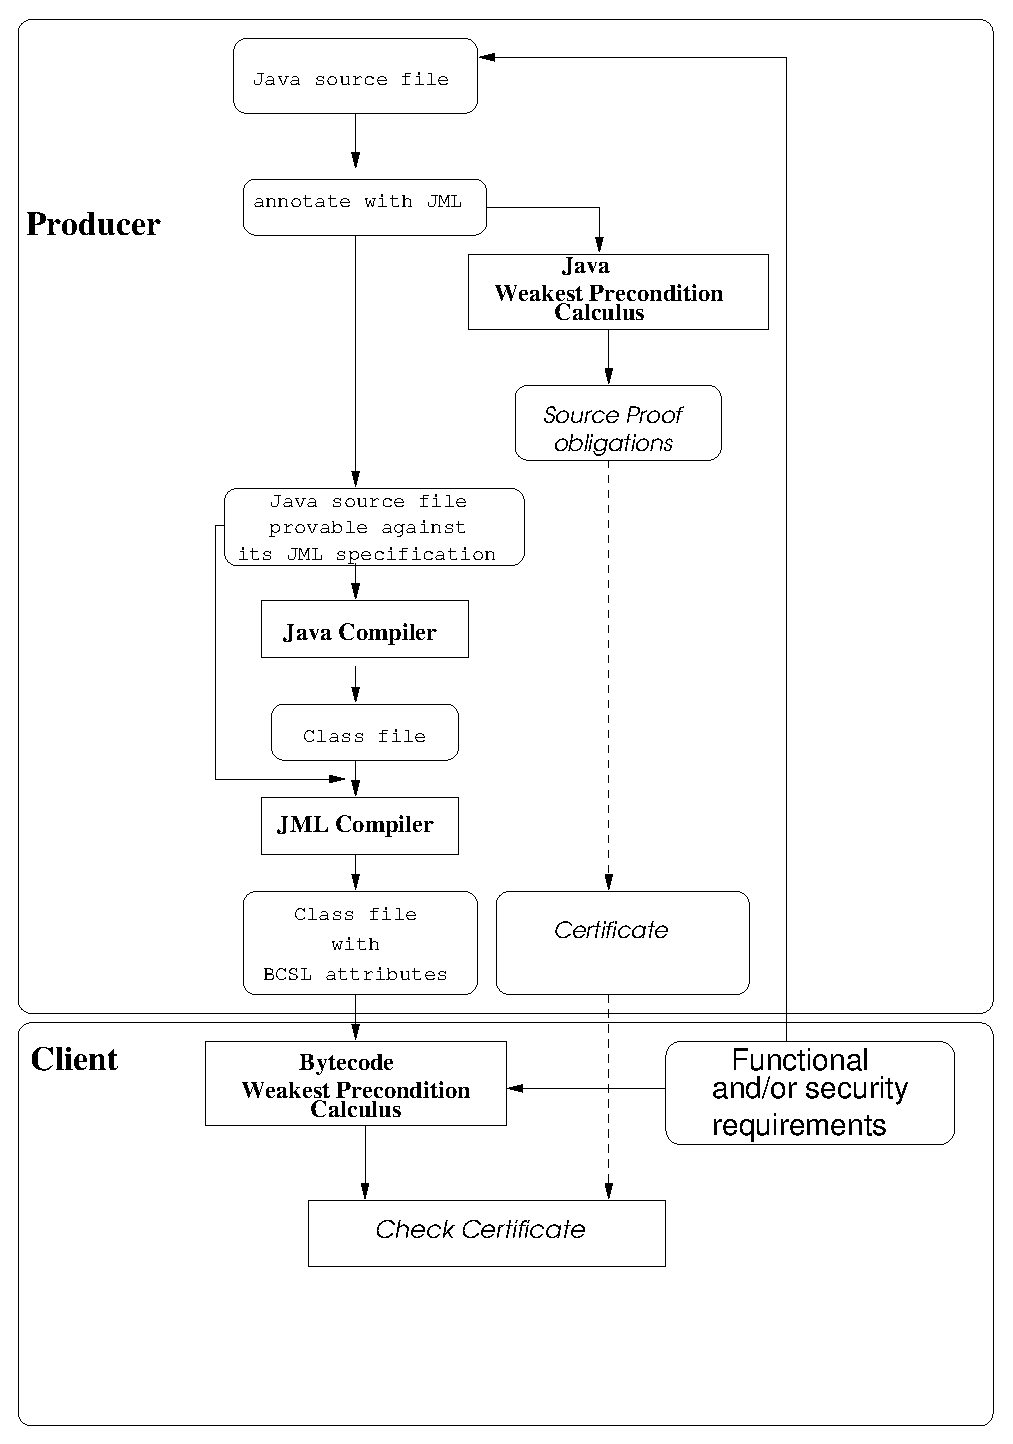
\epsfig{file=architecture.eps, width=\linewidth}
\caption{The overall architecture for annotating and verifying code}
\label{architecture}
\end{center}
\end{figure}
%\clearpage

It describes a process that allows a client to trust a code produced by an untrusted code producer.

In the first stage of the process the client provides the functional and (or) security requirements to the producer. The requirements can be in different form:
\begin{itemize}
\item A specified interface that describes the application to be developed. In that case, the client has fully specified in JML the features that have to be implemented by the code producer.
\item An API with some restricted access to some method. In this case, the client can protect its system by restricting its usage (for example, if the client API provides transaction management facilities, a requirement can be for no nested transactions and the API method \texttt{open} for opening and method \texttt{close} for closing transactions can be annotated to ensure that \texttt{close} should not be called if there is no transaction running and \texttt{open} should not be called if there is already a running transaction).   
\end{itemize}

%OLD:
% In the development process, the producer uses Jack to check the client requirements and usually has to add JML annotations for this %In both cases, the code producer develops its application and proves that it fulfills the given requirements using Jack; %in most cases, to complete this task, some annotations have to be added to the code 
%e.g. loop invariants, class invariants, method preconditions and postconditions etc. In a standard, application only after specifying enough the source code, 
%have we got the annotated Java source files to feed to the JML compiler.

In the development process, the producer verifies if the client requirements are respected by generating verification conditions
over the source code and usually, he has to add JML annotations for this e.g. loop invariants, class invariants, method preconditions
 and postconditions etc. Usually, only after specifying enough the source code, 
have we got the annotated Java source files to feed to the JML compiler.



When the annotations are sufficient to prove the code, 
the Java file is then normally compiled with a Java compiler to obtain a 
class file. This class file is then extended with user defined attributes that contain the BCSL specification, resulting from the compilation of the JML specification. 
At this stage, the Java class files contain all the information that will allow the client to check it. 
 %OLD
%In particular, the client will generate proof obligations from the untrusted annotated bytecode and his security requirements 
%(expressed in a suitable form) as shown in figure~\ref{architecture}. Proof obligations are formulas which, if provable, guarantee the bytecode correctness.
%The latter are then proved , for instance, with JACK (see section \ref{prelim}). If the client succeeds in proving 
%the verification conditions, he can trust the unknown code. Currently the framework does not support sending both the proof and the 
%bytecode to the client, which is the next step in our work.
In particular, the client will generate proof obligations from the untrusted annotated bytecode and his security requirements 
(expressed in a suitable form) as shown in figure~\ref{architecture}. Proof obligations are formulas which, if provable, guarantee the bytecode correctness.
The latter are then proved with a theorem prover (possibly interactively). If the client succeeds in proving 
the verification conditions, he can trust the unknown code. Currently the framework does not support sending both the proof and the 
bytecode to the client, which is the next step in our work.

%OLD
%To implement this architecture, we have defined a compiler from JML to BCSL; the JML compilation results in an extension of the class file format; 
%we have implemented a tool to insert those special attributes in the class file and we have extended the JACK framework to generate proof obligations at bytecode 
%level and to prove them with the plugged JACK provers (as explained in the introduction). 
%The coming sections introduce those features.  

To implement this architecture we use JACK as a verification condition generator both on the consumer and the
producer side. JACK is a plugin for the eclipse\footnote{http://www.eclipse.org} integrated development environment for Java. Originally, the tool was designed as verification condition generator for Java source programs against their JML specification. JACK can interface with several theorem provers (AtelierB, Simplify, Coq, PVS). We have extended the tool with a compiler from JML to BCSL and a bytecode verification condition generator. In the following we introduce the BCSL language, the JML compiler and the bytecode weakest precondition calculus which underlines the bytecode verification condition generator.
 
%the JML compilation results in an extension of the class file format; we have implemented a tool to insert those special attributes in the class file and we have extended 
%the JACK framework to generate proof obligations at bytecode level and to prove them with the plugged JACK provers (as explained in the introduction). 
%The coming sections introduce those features.  

% CHANGED - the example o compilation of loop specification

\section{Bytecode Specification Language (BCSL)}\label{bcSpecLg}
%Traditionally a lot of research has been done in the field of program verification for structured program languages~\cite{WPCDS},
%~\cite{DisDij}. This explains the fact that the existing specification languages are designed for dealing with high level program languages. 
In this section, we propose a bytecode specification language which we call BCSL. We define a compiler from the high level specification language JML to BCSL. The specification compilation results in a class file extension. In the following we give the grammar of BCSL and sketch the specification compiler.

%In order to verify 
%a program w.r.t. to some property, usually the property is expressed in a suitable specification language.
%After compilation, the executable code is detached from the source code; still there are situations where the bytecode is subject to verification procedures (e.g. for example establishing trust in it). A typical example is when an untrusted bytecode implementing a public interface arrives at a 
%receiver side and the latter wants to check that the unknown  bytecode respects the interface specification (which may not be trivial).
% Here comes the need for writing specification on  bytecode level.


\subsection{Grammar} \label{grammar}
We propose a bytecode level specification language which corresponds to a representative subset of JML.
We sketch the bytecode specification language grammar in fig.~\ref{bclGrammar}. We omit some of the definitions 
because of space constraints, e.g. the grammar for arithmetic expressions (which is defined in a standard way). For the full specification we refer to ~\cite{JML2BCSpec}.  
\begin{figure}[!htbp]
$$ \begin{array}{l}
\ClassSpec ::= \jmlStmt{class \ invariant} \ \predicate \\
     \Myspace \Myspace \Myspace \Myspace \Myspace  \mid  \jmlStmt{history \ constraint} \ \predicate \\
     \Myspace \Myspace \Myspace \Myspace \Myspace  \mid  \jmlStmt{model} \ \texttt{ClassName}  \ id \\
      \\
\MethodSpec  ::= \SpecCase \\
   \Myspace \Myspace \Myspace \Myspace \Myspace \Myspace  \mid  \SpecCase \  \jmlStmt{also} \  \MethodSpec	;\\
   \\
\SpecCase ::= \jmlStmt{requires} \ \predicate;\\ 
	\Myspace \Myspace \Myspace \Myspace  \Myspace \mid  \jmlStmt{modifies} \ list(\expression);\\
	%\Myspace \jmlStmt{decreases} \ \expression;\\
    \Myspace \Myspace \Myspace \Myspace \Myspace \mid  \jmlStmt{ensures} \ \predicate;\\
    \Myspace \Myspace \Myspace \Myspace \Myspace \mid  \jmlStmt{exsures} \ (\texttt{ExceptionClass}) \ \predicate;\\
                     \\
\interMethodSpec ::= \loopSpec \\
	 \Myspace \Myspace \Myspace \Myspace \Myspace \Myspace \Myspace \Myspace  \mid \assert \\
	  \\
\loopSpec ::= \jmlStmt{pc\_ index} \ int;\\
	    \Myspace \Myspace \Myspace \Myspace \Myspace \mid \jmlStmt{loop\_modifies} \ list(\expression);\\
       \Myspace\Myspace \Myspace \Myspace  \Myspace \mid \jmlStmt{loop\_invariant}  \ \predicate; \\
	   \Myspace \Myspace \Myspace \Myspace \Myspace \mid \jmlStmt{loop\_decreases} \ \expression; \\
	 \\								
\assert   ::= \jmlStmt{pc\_ index} \ int;\\
		\Myspace \Myspace \Myspace \Myspace \mid \jmlStmt{assert} \ \predicate; \\
	\\

      \predicate ::= \true \ \mid \ \false \\
      \Myspace  \Myspace \mid   \expression \ predSymbol \ \expression \\
       \Myspace \Myspace \mid   \predicate \wedge \predicate \\
       \Myspace \Myspace \mid   \predicate \vee \predicate \\
       \Myspace \Myspace \mid   \predicate \Rightarrow \predicate \\
       \Myspace \Myspace \mid   \forall (\texttt{boundVar } : JavaType )  \predicate \\
       \Myspace \Myspace \mid   \exists(\texttt{boundVar } : JavaType )  \predicate \\
       \\ 
  \expression ::= \ArithExpr  \mid  \ \register{i}  \  \mid  \ \reference \\
  	  \Myspace \Myspace  \mid  \ \fieldAccess{\expression}  \\
  	  \Myspace \Myspace  \mid \ \arrayAccess{\expression} {\expression}  \\
  	  \Myspace \Myspace  \mid \result \ \mid \old{\expression} \mid \ \EXC \\
  	  \Myspace \Myspace \mid \typeof{\expression}  \ \mid \ \Mynull \ \mid \ \this \\
  	  \Myspace  \Myspace \mid  \counter \mid \stack{\ArithExpr} \ldots
\end{array}$$
\caption{BCSL grammar}
 \label{bclGrammar}
 \end{figure}
 The language defined here is expressive enough for most purposes including the description of non trivial functional and 
 security properties. We now discuss some of the specification clauses that have some differences with JML, for the rest their semantics is the same as in JML and can be found in~\cite{RT03djml,JMLRefMan}.
 
 We can specify using the specification clause \jmlKey{exsures} what is the postcondition of  a method in case it terminates with 
 an exception  \texttt{E}. If the postcondition states something about the exception object thrown then the special expression \texttt{EXC} is used 
(this expression can appear only in exceptional postconditions). If \jmlKey{exsures} is not specified for certain exception, then by default it is considered as \Myfalse.
 
As shown by the grammar, BCSL allows us to specify different method specification cases separated by the keyword \jmlKey{also} --- this means that 
 method caller has to satisfy the disjunction of the preconditions in the specification cases  and the method's implementation 
 has to guarantee the postcondition of every specification case of which the precondition held in the prestate.

Loop specifications and assertions are tagged with the program point in the bytecode where they must hold. Among the expressions that are handled (almost all are also handled
by JML) we have $\counter$ and \stack{\ArithExpr} which respectively stand for the stack counter and an element on the stack at position \ArithExpr. These expressions do not appear in the precondition and postcondition specification of a method. Later we shall see how they are used.
 
 
\subsection{Compiling JML into bytecode specification language}\label{comJML}

This section explains how JML specifications are compiled into bytecode level specifications and how they are inserted into the bytecode. 
 
Before going farther we give a brief description of the class file format. As defined by the Java Virtual Machine Specification (JVMS) \cite{VMSpec}, a class file contains a definition of a single class class or interface. It contains information about the class name, interfaces implemented by the class, super class, methods and fields declared in the class and references. The JVMS mandate that the class file contains data structure usually referred as the \textbf{constant\_pool} table which is used to construct the runtime constant pool upon class or interface creation. The runtime constant pool serves for loading, linking and resolution of references used in the class. The JVMS allows to add to the class file a user specific information(~\cite{VMSpec}, ch.4.7.1). This is done by defining user specific attributes  (their structure is predefined by JVMS).

Thus the ``JML compiler'' \footnote{Gary Leavens also calls his tool jmlc JML compiler, which transforms jml into runtime checks and thus generates input for the jmlrac tool  } compiles the JML source specification into user defined attributes. The compilation process has three stages:
\begin{enumerate}
\item compile the Java source file. This can be done by any Java compiler that supplies for every method in the generated class file the \textbf{Line\_Number\_Table} and \textbf{Local\_Variable\_Table}  attributes. The presence in the Java class file format of these attribute is optional \cite{VMSpec}, yet almost all standard non optimizing compilers can generate these data. The \textbf{Line\_Number\_Table} describes the link between the source line and the bytecode of a method.  The \textbf{Local\_Variable\_Table} describes the local variables that appear in a method. This attribute is important for the next phase of the JML compilation.
\item from the source file and the resulting class file compile the JML specification. In this phase Java and JML source identifiers are linked with their identifiers on bytecode level, namely with the corresponding indexes either from the constant pool or the array of local variables described in the \textbf{Local\_Variable\_Table} attribute. It is also in this phase that the specification parts like the loop invariants and the assertions which should hold at a certain source program point must be associated to the respective program point on bytecode level. The specification
is compiled in binary form using tags in the standard way. Basically the compilation of an expression is a tag followed by the compilation of its subexpressions. 
Thus for example the loop invariant specified in JML for the method \texttt{replace} in Fig.~\ref{replaceSrc} is :
$$
\begin{array}{l}
\register{3} \le length(\#19(\register{0})) \ \wedge \\
\register{3} \ge 0  \ \wedge \\ 
       \forall  var_0 \in int . \left(\begin{array}{l} 0 \le var_0 \ \wedge \\ var_0 < \register{3}  \\
                \Rightarrow  \#19(\register{0})[var_0] \neq \register{1} \end{array} \right)
\end{array}
$$
From the example one can see that local variables and  fields are respectively linked to the index of the register table for the method and to the corresponding index of the constant pool table (\#19 is the compilation of the field name \texttt{list}, \register{3} stands for the method local variable \texttt{i}). 
\item add the result of the JML compilation in the class file as user defined attributes. Method specifications, class invariants, loop invariants are 
newly defined attributes in the class file.
 For example, the specification of all the loops in a method are compiled to a unique method attribute: whose syntax is given in fig.~\ref{loopAttribute}. This attribute is an array of data structures each describing a single loop from the method source code. Also for each loop in the source code there must be a corresponding element in the array. 
More precisely, every element contains information about the instruction where the loop starts as specified in the \textbf{Line\_Number\_Table}, the invariant associated to this loop, the decreasing expression in case of total correctness, the expressions that can be modified. 
For the full specification of the compiler one can see~\cite{JML2BCSpec}.
\end{enumerate}

\begin{figure}[ht!]
\textbf{     
\begin{tabbing}
JML\=Loop\_specification\_attribute \{\\
\> ...\\
\> \{\hspace{3 mm}\= u2 index;\\
\> \> u2 modifies\_count;\\
\> \> formula modifies[modifies\_count];\\
\> \> formula invariant;\\
\> \> expression decreases;\\
\> \} loop[loop\_count];\\
\}
\end{tabbing}
}

\begin{itemize}
\item \textbf{index}: The index in the  \texttt{LineNumberTable } where the beginning of the corresponding loop is described

\item \textbf{modifies[]}: The array of modified expressions.

\item \textbf{invariant }: The predicate that is the loop invariant. It is a compilation of the JML formula in the low level specification language

\item \textbf{decreases}: The expression whose decreasing at every loop iteration will guarantee loop termination 
\end{itemize}
\caption{Structure of the Loop Attribute}
\label{loopAttribute}
%\end{frameit}
\end{figure}

The JML compiler does not depend on any specific Java compiler, but it requires the presence of a debug information, namely the presence of the \textbf{Line\_Number\_Table} attribute for the proper compilation of inter method specification, i.e. loops and assertions. We think that this is an acceptable restriction for the compiler. The most problematic part of the compilation is to find the program points where the loop invariants must hold. This basically means that one has to identify which source loop corresponds to which bytecode loop in the control flow graph. To do this, we assume that the control flow graph is reducible~\cite{ARUCom1986} (intuitively this means no jumps from outside a loop inside it); graph reducibility allows to establish the same order between loops in the bytecode and source code level and to compile correctly the invariants to the proper places in the bytecode.


\todo{limitations : registers that are used with two different types in the method bytecode}


\section{Weakest Precondition Calculus For Java Bytecode}\label{wpbc}
In this section, we define a bytecode logic in terms of a weakest precondition calculus.
We assume that the bytecode program has passed the bytecode verification procedure (we discuss the issue in section \ref{relWork}),
 thus the calculus is concerned only with program functional properties. We also assume that code is generated by a non optimizing compiler. 

The proposed weakest precondition has those features:
\begin{itemize}
%\item modular, design by contract verification, in particular every method is verified separately method calls being translated to their specification 
\item it supports all Java sequential instructions except for floating point arithmetic instructions and 64 bit data (\java{long} and \java{double} types), including 
exceptions, object creation, references and subroutines. The calculus is defined over the method control flow graph

\item it supports BCSL (section \ref{bcSpecLg}), i.e. method's specification written in BCSL like pre- and postconditions, assertions at particular program point among 
which loop invariants (if there is nothing special specified the specification by default: preconditions, postconditions and invariants are taken to be true) is taken into account. %The verification procedure assumes that the bytecode is specified enough, i.e. we do not try to infer specification, as we assume that they are compiled from the source program
\end{itemize}

The calculus is defined over the control flow graph of the program and has two levels of definitions --- the first one is the set of rules for single Java bytecode instructions (discussed in subsection~\ref{wpInstr} ) and the second one takes into account how control
 flows in the bytecode(subsection ~\ref{wpGraph}). A related problem is how the loops in the control flow are treated. 
As we mentioned earlier we assume that every method is specified in sufficient details, i.e. if there are loops, the corresponding 
loop invariant is present. This allows us to ``cut'' the loops in the graph at the program point where the invariant must hold. 
These ``cuts'' generate an abstract control flow graph which is acyclic and over which the verification conditions are generated. Subsection ~\ref{abstrCntrFlow} discusses 
how the abstract control flow graph is generated.

%In the rest of the section we describe the bytecode logic  and how the verification conditions are generated:
% the weakest precondition rules for single Java bytecode instructions in subsection \ref{wpInstr}, 
% the method abstract control flow graph is explained in subsection ~\ref{abstrCntrFlow}, 
% the definition of the weakest precondition over the abstract control flow graph is discussed in ~\ref{wpGraph} where how exception handling and subroutines
%are described.



\input wpSingleInstr.tex
\input abstractCntrFlow.tex
\input wpOverGraph.tex

%\begin{center} \texttt{wp} : \texttt{STMT} $\longrightarrow$ \texttt{Predicate} $\longrightarrow$ \texttt{Predicate}\end{center}






%\subsection{Weakest Precondition Function for bytecode \\instructions}\label{wpInstr}
%We define a weakest precondition (\wpi) predicate transformer function which takes into account normal and exceptional termination. 
%\wpi \ takes three arguments: an instruction, a predicate that is the instruction's normal postcondition $\psi$, and a function
%from exception types to predicates $\excPost$ (it returns the specified postcondition in the \jmlKey{exsures} clause for a given exception; see section~\ref{grammar}).
%The \wpi \ function returns the weakest predicate such that if it holds in the state when the instruction starts its execution the following conditions are met: 
%\begin{enumerate}
	% \item if the instruction terminates its execution normally the predicate $\psi$ holds in the poststate 
	% \item if it terminates with an exception \texttt{E} then the predicate $\excPost(\tt{E})$ holds in the poststate.
%\end{enumerate}


 
 %The instruction $\instr{Type\_load} \ i$ loads on the top of the stack the value of the method local variable at index \textit{i}
 %in the \textbf{Local\_Variable\_Table} (see section~\ref{bcSpecLg}).

%As we said in the beginning of the section, \wpi \ ``understands'' the bytecode specification language, i.e. the keywords have their 
%corresponding semantics. For example, the keyword \result \ is evaluated only by \instr{Type\_return} 
%instructions and if appearing in the postcondition, \result \ is substituted by the element on the top of 
%the stack \stack{\counter}. 

%The rules also take into account the possible abnormal execution of the instruction. For example, in Fig. \ref{instrWP}, the rule for the instruction \instr{putField}
%has two conjuncts - one in the case when the dereferenced object is not null and the instruction execution terminates normally; the other one stands for the case when this is not true. Note, in case the exception thrown is not handled, we substitute the special specification variable \jmlKey{EXC} with the thrown exception object.


%\begin{figure}[!htp]
%$$
% (\texttt{Cl.f})\oplus[e2 \rightarrow e1](o) = \left\{ \begin{array} {ll}
%						       e1 & if \ e2 = o \\
%					               \texttt{Cl.f}(o)	& else 
%	\end{array}\right. 
%$$ 
%\caption{Overriding Function}
%\label{override}
%\end{figure}

\subsection{Manipulating object fields}
Instance fields are treated as functions, where the domain of a field \texttt{f} 
declared in the class \texttt{Cl} is the set of objects of class \texttt{Cl} and its subclasses.
We are using function update when assigning a value to a field reference as, for instance in~\cite{B00ppp}. In Fig.\ref{instrWP}, we give the \wpi \ rule for the
instruction \instr{putfield} \texttt{Cl.f}, which updates the field \texttt{Cl.f}\footnote{ \texttt{Cl.f} stands for the field \texttt{f} declared in class 
\texttt{Cl}} of the object referenced by the reference stored in the stack below the stack top \stack{\counter-1} with the value on the stack top \stack{\counter}.
 Note that the rule takes in account the possible exceptional termination.
%In Fig.~\ref{instrWP} the rule for \instr{putField} substitutes the corresponding field function \texttt{Cl.f} with \texttt{Cl.f} updated for object $o$, in case the dereferenced object is not null. The definition of update function is given in figure~\ref{override}.


%To illustrate how references are treated we give an example at fig.\ref{aliasing} - a method that assigns to the parameter's instance integer field (we give the example in source code to keep simplicity). 
%The \wpi \ for the method is given at      

%\begin{figure}
%\begin{verbatim}
%public class FieldAssign {
%  public int i = 0;

 % //@requires a != null;
 % //@modifies a.i; 
  %//@ensures i == 5;
 % public void set( FieldAssign a) {
 %   a.i = 3;
 % } 
%}
%\end{verbatim}
%%\caption{Example for recursive Java class}
 %\label{aliasing}
%\end{figure}

\subsection{Method calls}
Method calls are handled by using their specification. A method specification is a contract between callers and callees --- the precondition of the called method
must be established by the caller at the program point where the method is invoked and its postcondition is assumed to hold after the invocation. The rule for
invocation of a non-void instance method is given in Fig.~\ref{wpInv}. In the precondition of the called method, the formal parameters and the object on which the method is called are substituted with the first \textit{n+1} elements from the stack top. 
Because the method returns a value, if it terminates normally, any occurrence of the JML keyword \result \ in $\psi^{post}(m)$ is substituted with the fresh variable $fresh\_var$.  
Because the return value in the normal case execution is put on the stack top, the $fresh\_var$ is substituted for the stack top in $\psi$. The resulting predicate is quantified over the expressions that may be modified by the called method. We also assume that if the invoked method terminates abnormally, by throwing an exception of type $\texttt{Exc}$, on returning the control to the invoker its exceptional postcondition $\excPost_{\tt{m} }( \tt{Exc} )$ holds. 
The rule for static methods is rather the same except for the number of stack elements taken from the stack.  

\begin{figure}[!ht]
$$
\begin{array}{l}
\wpi(\instr{invoke \  m}, \ \psi ,\ \excPost) =\\ 
\begin{array}{l}
\Myspace \psi^{pre}(m) \ \wedge \\
\Myspace  \forall_{j = 1..s} e_{j}.\biggl( 
\Myspace \psi^{post}( \texttt{m}) 
                     \begin{array}{l}
                     \substitution{\register{i}}{\stack{\counter+i-nArg(\texttt{m}) }}_{i=0}^{\tt{nArg(m)}}  \\
                      \substitution{\tt{\backslash result} }{ fresh\_var } \\
                     \end{array} \\
  \Myspace\Myspace\Myspace\Myspace\Myspace                    \Rightarrow  \\
\Myspace\Myspace\Myspace\Myspace\Myspace   \psi  \begin{array}{l}
                             \substitution{\counter }{\counter - \tt{nArg}( \texttt{m} )} \\
                             \substitution{\stack{\counter } }{ \tt{fresh\_var}}  \   
                         \end{array}\biggr) \\
\wedge_{i = 1}^k\\
\Myspace \forall_{j = 1..s} e_i \biggl( 
\Myspace \excPost_{\tt{m} } ( \tt{Exc_i} ) \\
\Myspace\Myspace\Myspace\Myspace\Myspace \Rightarrow \\
\Myspace\Myspace\Myspace\Myspace\Myspace   \excPost(\tt{Exc_i} )
                                 \begin{array}{l}
                                       \substitution{ \counter}{  0} \\
                                        \substitution{\stack{0}}{ \stack{\counter}}   
              		\end{array}   \biggr)   \\
\end{array} \\[15 mm]
\end{array}
$$
$\psi^{pre}(\texttt{m})$ -  the specified  precondition of  method \texttt{m} \\
$\psi^{post}(\texttt{m})$ - the   specified   postcondition   of   method  \texttt{m}  \\
$\excPost_{\texttt{m}}$ - the   exceptional   function   for   method  \texttt{m}  \\
\texttt{nArg}( \texttt{m} ) -  the    number   of   arguments   of   \texttt{m} \\  
$e_{j} , j = 1 .. s$ - the   locations   modified   by   method   \texttt{m} \\
$\tt{Exc_i}, i = 1..k$ -  the   exceptions   that  \texttt{m} may  throw \\


\caption{\sc \wpi \ rule for a call to an instance non void method}
\label{wpInv}
\end{figure}


\section{Comparison between source and bytecodes \\ proofs}  \label{results}

The purpose of this section is to give a comparison between bytecode and source proof obligations.
In particular, we illustrate this by the proof obligations of the example program in Fig.\ref{replaceSrc}.
%We have an implementation of the JML compiler ( subsection \ref{comJML}) and the bytecode verification condition generator based on the weakest precondition calculus (Section \ref{wpbc}) which are integrated in JACK. Both of the verification condition generators perform the same simplifications over the verification conditions 
%, e.g. eliminate verification conditions that contain contradictory hypothesis or trivial goals (equal to true). 

%The performed tests show that JML compilation augments around twice the file size. 
%For the example in Fig.~\ref{replaceSrc}, the class file without the specification extensions is 548 bytes, 
%and the class with the BCSL extension BCSL is 954 bytes. 
%The size of the bytecode specification is proportional to the source specification: 
%the bigger is the source specification, the greater will be the size of the class file. 
We studied the relationship between the source code proof obligations generated 
by the standard feature of JACK and the bytecode proof obligations generated by our implementation over the corresponding bytecode
 produced by a non optimizing compiler over the examples given in \cite{JPVC03JKM}. The proof obligations were the same modulo 
program variables names and basic types.

 We return now to our example from the previous sections and give in Fig. \ref{vcEnsures} one of the proof obligations on source 
and bytecode level respectively concerning the postcondition correctness. The verification conditions on bytecode and source level
 have the same shape modulo names (see Section \ref{comJML} for how names are compiled). Also in Section
 \ref{comJML}, we discussed the compilation of the JML postcondition from Fig. \ref{replaceSrc}. Particularly,
 we saw that the compiler has to transform the source postcondition in an equivalent formula and we
 gave the compilation in Fig. \ref{postCompile}. 

Despite those transformations, the source and bytecode goal respectively (which are actually the postcondition) on bytecode and source level are not only
semantically equivalent but syntactically the same (except for the variable names ). Still, in the bytecode proof obligation we have one more hypothesis than on source level. The extra hypothesis in the bytecode proof obligation is related to the fact that the result type is boolean but the JVM encodes boolean expressions as integers (which is trivially true). This means that the proof obligations have also the same shape.

 Another important issue is the impact of simple optimizations like dead code elimination on the relationship between source and bytecode proof obligations. 
In this case, the compiler does not generate the dead code and the bytecode verification condition generator will neither ``see'' it. 
Even though the source contains the never taken branch as the condition is equivalent to false, this will result in a trivially true
verification condition which the JACK source verification condition generator will discard.

The equivalence between source and bytecode proof obligations can be exploited in PCC scenarios, as we discussed in Section \ref{architecture} where 
the producer generates the program certificate over the source code in scenarios where a complete automatic certification (e.g. the certifying compiler) will not work.
 
We aim to formally give evidence that the proof obligations on non optimized bytecode and source programs are syntactically the same (modulo names and types). 

%Fig. \ref{vcLoopPreserv} shows the proof obligations for the loop preservation. As you can see the hypothesis and the goal have the same ``shape'' on bytecode and source code and the differences are due to the variable names.



% \begin{figure}{!h}

% $$\begin{array}{ll}
%Hypothesis \ on \ bytecode:  & Hypothesis \ on \ source \ level:  \\
%% & \\

%
%\begin{array}{l}
% \register{1} \neq \\
%\#19 (\register{0})[\register{2}\_at\_ins\_22]
%\end{array}  
%
%&  
%\begin{array}{l}
% \srcVar{obj} \neq \\
%  ListArray.list(\this)[\srcVar{i}\_at\_ins\_26] 
%\end{array}   \\
%
%
%
% & \\
%
%\#19(\register{0}) \neq \Mynull &  ListArray.list( \this) \neq \Mynull\\
%
%
%& \\
%
%\begin{array}{l}
%  len(\#19 (\register{0})) > \\
% \register{2}\_at\_ins\_22 
%\end{array}
%%& 
%\begin{array}{l}
%  len(ListArray.list(\this)) > \\
%\srcVar{i}\_at\_ins\_26
%\end{array}         \\ 

%

% & \\
%
% \register{2}\_at\_ins\_22 \geq 0 &   \srcVar{i}\_at\_ins\_26    \geq 0    \\
%
%
% & \\
%\begin{array}{l}
%  \register{2}\_at\_ins\_22 < \\
%  len(\#19(\register{0}))
%\end{array} &
%
%\begin{array}{l}
%  \srcVar{i}\_at\_ins\_26 <\\
%  len(ListArray.list(\this))
%\end{array}   \\
%
%
% & \\
%\begin{array}{l}
%  \register{2}\_at\_ins\_22 \leq \\
%  len( \#19(\register{0}))
%\end{array} 
%&  
%\begin{array}{l} 
%  \srcVar{i}\_at\_ins\_26 \leq \\
%  len(ListArray.list(\this))
%\end{array}   \\
%
%
% &\\
%% \register{2}\_at\_ins\_22 \geq 0 &   \srcVar{i}\_at\_ins\_26 \geq 0 \\
%
%
%
%% &\\
% \begin{array}{l} 
%         \forall  var(0). \ 0 \leq var(0) \wedge var(0) < (\register{2}\_at\_ins\_22) \Rightarrow \\
%                \Myspace    \#19(\register{0})[var(0)] \neq \register{1}
%      \end{array} &        
%      \begin{array}{l} 
%             \forall  var(0). \ 0 \leq var(0) \wedge var(0) < (\srcVar{i}\_at\_ins\_26) \Rightarrow \\
%                 \Myspace       ListArray.list(\this)[var(0)] \neq \srcVar{obj}
%      \end{array}  \\
%%
% typeof(\register{0}) <: ListArray &    typeof(this) <: ListArray     \\
%
%& \\
%& \\
%Goal \ on \ bytecode: & Goal \ on \ source \ level: \\
%
%& \\
%
%  \begin{array}{l}
%               1 + \register{2}\_at\_ins\_22 \leq  len(ListArray.list(\register{0}))  \\
%
%               1 + \register{2}\_at\_ins\_22 \geq 0 \\
%
%               \forall  var(0). 0 \leq var(0) \wedge var(0) < 1 + \register{2}\_at\_ins\_22 \Rightarrow \\
%                   \Myspace  ListArray.list(\register{0})[var(0)] \neq \register{1} 
%
%       \end{array}
%& 
%
%       \begin{array}{l}
%             1 + \srcVar{i}\_at\_ins\_26 \leq  len(ListArray.list(this))  \\
%	     \\
%             1 + \srcVar{i}\_at\_ins\_26 \geq 0 \\
%	     \\
%             \forall  var(0). 0 \leq var(0) \wedge\\
%	     \Myspace  var(0) < 1 + \srcVar{i}\_at\_ins\_26 \Rightarrow \\
%                  \Myspace  ListArray.list(this)[var(0)] \neq \srcVar{obj} 
%       \end{array}   
%
 
%\end{array}$$



%\caption{Source and Bytecode verification condition for loop preservation for method \texttt{ListArray.isElem} }
%\label{vcLoopPreserv}
%\end{figure}








\begin{figure*}[!h]

\begin{center}
\begin{tabular}{|l|l|}
\hline
\bf{Hypothesis \ on \ bytecode:}  & \bf{Hypothesis \ on \ source \ level:}  \\
\hline 
$\register{2}\_at\_ins\_20 \geq $ 
& $ \srcVar{i}\_at\_ins\_26 \geq$ \\

$len(\#19(\register{0})) $ & $  len(ListArray.list(\this)) $ \\
\hline 

$\#19(\register{0}) \neq \Mynull$ 
& $ ListArray.list(\this) \neq \Mynull$ \\

\hline 
$ \register{2}\_at\_ins\_20) \leq$ 
&  $  \srcVar{i}\_at\_ins\_26  \leq   $ \\
$ len(\#19(\register{0}))  $ & $ len(ListArray.list(\this))  $ \\
\hline

$\register{2}\_at\_ins\_20 \geq 0  $ 
& $ \srcVar{i}\_at\_ins\_26  \geq 0 $ \\

\hline

$\forall  var(0). \  0 \leq var(0) \wedge  $ & $\forall  var(0). \  0 \leq var(0) \wedge $ \\
$ var(0) < \register{2}\_at\_ins\_20 \Rightarrow $ & $  var(0) < \srcVar{i}\_at\_ins\_26 \Rightarrow $\\
$ \#19(\register{0})[var(0)] = \register{1}   $ & $  ListArray.list(\this)[var(0)] = \srcVar{obj}  $ \\

\hline

 $typeof(\register{0}) <: ListArray$ & $typeof( \this) <:  ListArray$  \\
\hline

$0=0 \vee 0=1$ & \\

& \\

\hline
\bf{Goal on bytecode:} & \bf{Goal on source level:} \\
\hline
$\Myfalse  \iff $ & $\Myfalse \iff  $ \\
 $ \exists  var(0) . \ 0 \leq var(0) \wedge$ 
& $ \exists  var(0) . \ 0 \leq var(0) \wedge$ \\

$\Myspace \Myspace var(0) < len(\#19(\register{0})) \wedge$ 
& $\Myspace \Myspace  var(0) < len(ListArray.List(this)) \wedge $\\
       
$\Myspace \Myspace \#19(\register{0})[var(0)] = \register{1} $ 
&$\Myspace \Myspace  ListArray.List(this)[var(0)] = \srcVar{obj}  $ \\

\hline
\end{tabular}
\end{center}

Note: $\expression\_at\_ins\_n$ denotes the value of  
expression $\expression$ at the bytecode instruction at index (source line)  $n$ 

\caption{\sc Comparison of source and bytecode verification conditions}
\label{vcEnsures}
\end{figure*}

\clearpage
 















%\subsubsection{Example}
% We give a simple example of how the \wpi \ works. Block $\blockm{6}$ (starts at instr. \texttt{6}) in Fig.~\ref{blockBC} ends with a branching instruction and in the case when the condition is true (the current element of the array is not equal to the first parameter of the method \texttt{replace}) the execution will continue at $\blockm{19}$. Below we give the part of the weakest precondition for block $\blockm{6}$ in case the control flows to block $\blockm{19}$( the condition of its last instruction holds and in this case 
%the predicate $pre(b^{6}, b^{19})$ is $\wpi(\blockm{19})$).  The implications with conclusion \Myfalse \ stand for the possible exceptions \texttt{NullPointer} and \texttt{ArrayIndexOutOfBound} exceptions that may be thrown (as no postcondition is specified explicitly for these cases of abnormal termination, the one by default is taken). 

%\input wpExample.tex

\section{Conclusion and Future Work}\label{conclusion}
This article describes a bytecode weakest precondition calculus applied to a bytecode specification language (BCSL).
BCSL is defined as suitable extensions of the Java class file format.
Implementations for a proof obligation generator and a JML compiler to BCSL have been developed and are part of the Jack 1.8 release\footnote{http://www-sop.inria.fr/everest/soft/Jack/jack.html}.
At this step, we have built a framework for Java program verification.
 This validation can be done at source or at bytecode level in a common environment: for instance, to prove lemmas ensuring bytecode correctness all the current and future provers plugged in Jack can be used.

We are now aiming to complete our architecture for establishing trust in untrusted code - in particular extending the present work to a PCC architecture for establishing non trivial requirements.  
%Properties that can be verified are properties expressible in the JML specification language. Design by contract properties (used in interface design) can be easily expressed and sent through a network with this framework. What should be pointed out is that we do not deal with such low level properties like for example memory allocation or time constraints.What the approach proposes is suitable for verifying static properties (invariant) concerning objects: it can be relations between values, or conditions over expressions that the program treats.
In this way, several important directions for future work are:
\begin{itemize}
\item perform case studies and strengthen the tool with more experiments.
\item find an efficient representation and validation of proofs in order to construct a PCC framework for Java bytecode. We would like to build a PCC framework where the proofs are done interactively over the source code
and then compiled down to bytecode. Actually, as we stated in Section \ref{results} the proof obligations generated over a source program and over its compilation with non optimizing compiler are syntactically equivalent modulo name and types. 
\item an extension of the framework applying previous research results in automated annotation generation for Java bytecode (see~\cite{PBBHL}). The client thus will have the possibility to verify a security policy by propagating properties in the loaded code and then by verifying that the code verify the propagated properties.
%\item correctness of the semantics of the weakest precondition calculus proposed, which we will do over the bytecode operational semantics. 

\end{itemize}
%Finally, we are currently proving the correctness of the semantics of the weakest precondition calculus proposed, the proof is built over the bytecode operational semantics and will ensure the soundness of our weakest precondition calculus.



